% Chapter Template

\chapter{Introducción a la física del magnetismo en los sistemas biológicos} % Main chapter title

\label{sistemasBiologicos} % Change X to a consecutive number; for referencing this chapter elsewhere, use \ref{ChapterX}


%----------------------------------------------------------------------------------------

%----------------------------------------------------------------------------------------
%	SECTION 1
%----------------------------------------------------------------------------------------



"La vida en la Tierra ha evolucionado en un mar de campos electromagnéticos naturales. Durante el siglo pasado, este ambiente natural ha cambiado en forma significativa con la aparición de un vasto y creciente espectro de campos producidos por el hombre. Razonando a partir de modelos basados en la termodinámica de equilibrio y en efectos térmicos, al principio se pensó que esos campos artificiales eran demasiado débiles como para interactuar con los sistemas de moléculas biológicas y por tanto incapaces de influir sobre las funciones fisiológicas. Numerosos estudios de laboratorio se efectuaron para buscar efectos biológicos a nivel celular y molecular de campos electromagnéticos de diferentes frecuencias de oscilación, focalizándose en exposiciones que no producen efectos térmicos. Una conclusión que se desprende claramente de estos estudios es que muchas de las interacciones observadas no se basan en el calentamiento de los tejidos. Los campos electromagnéticos débiles pueden modular eventos químicos que ocurren en la superficie de la célula, amplificando los efectos de la fijación de hormonas, anticuerpos y neurotransmisores en sus correspondientes sitios receptores en las membranas. Los iones calcio juegan un rol clave en esta amplificación. Estos estudios fundamentan nuevos conceptos de comunicación entre células a través de las barreras constituidas por las membranas celulares. Señalan, con creciente certidumbre, a una organización esencialmente física de la materia viva, a un nivel mucho más fino que el correspondiente a la imagen estructural y funcional definida en la química de las moléculas\citep{RossAdey}.”

"No se ha alcanzado todavía una comprensión a fondo de los efectos biológicos de los campos electromagnéticos. El amplio espectro de temas que deben ser estudiados incide en el lento progreso hacia ese fin último. Entre las disciplinas involucradas están la biología básica, la ciencia médica y la práctica clínica, la ingeniería biológica y la ingeniería eléctrica, la química básica y la bioquímica, y la física fundamental y la biofísica. Los fenómenos estudiados abarcan extensos intervalos de escalas de espacio y de tiempo. Así, en un extremo, se tienen corrientes continuas y oscilaciones con longitudes de onda de más de 100 km, grandes organismos biológicos y corrientes alternas con períodos de milisegundos. En el otro extremo se tienen campos con longitudes de onda sub-milimétricas y períodos por debajo de 10-12 s, estructuras sub-celulares y moléculas de dimensiones sub-nanométricas, y tiempos característicos tan cortos como 10-15 s (o menos) de las reacciones bioquímicas\citep{Greenbaum}.

\section{Introducción}

El propósito de este capítulo es conectar la física del magnetismo con el estudio de algunos procesos fisiológicos en los organismos.

En biología se trabaja con un conjunto de niveles estructurales, cada uno de los cuales se sustenta en los niveles que lo preceden. Una mirada a los procesos biológicos desde la perspectiva del bio-electromagnetismo permite distinguir cuatro niveles:

En la base, un primer nivel atómico-molecular. Se estudia desde el punto de vista de la física cuántica. Generalmente se utiliza la ecuación de Schrödinger con términos que tienen en cuenta las interacciones eléctrica y magnética en los átomos y entre los átomos en las moléculas y entre las moléculas. Es el bien conocido nivel físico microscópico.

Un segundo nivel corresponde a estructuras supramoleculares y sus procesos.
Se estudian con herramientas de física estadística y de cinética física, teniendo en cuenta las interacciones eléctricas y magnéticas, así como los resultados de la investigación de las estructuras y los procesos en el nivel previo. Es el nivel físico mesoscópico. Se describen conjuntos numerosos a átomos y moléculas, cuyas dimensiones son grandes respecto de las distancias entre los átomos, pero son pequeñas respecto de las dimensiones características de los patrones de estructura (macroscópicos) que aparecen en el siguiente nivel.

Un tercer nivel, ya macroscópico, corresponde a la célula considerada como una unidad de estructura y función. Aquí se incluyen organismos unicelulares, como las bacterias.
Los procesos a este nivel se estudian, desde un punto de vista fisicoquímico, con la ayuda de modelos basados en la termodinámica de los sistemas fuera del equilibrio.
En las ecuaciones que relacionan los flujos con las fuerzas termodinámicas se incluyen los efectos de los campos eléctricos y magnéticos.

Los parámetros correspondientes los modelos formulados a este nivel se interpretan mediante estructuras y procesos pertenecientes a los dos niveles precedentes.

Finalmente, un cuarto nivel que corresponde al organismo en su totalidad, con sus tejidos y órganos. Ahora el estudio se lleva a cabo con las herramientas del electromagnetismo clásico de medios continuos. Cuando se construyen modelos matemáticos de tejidos desde una perspectiva embriológica o fisiológica, algunas veces el nivel celular se trata como si fuera mesoscópico y el cuarto nivel como macroscópico.

Las ecuaciones de Maxwell con sus parámetros fenomenológicos (permitividad dieléctrica, permeabilidad magnética y conductividad eléctrica) se aplican a modelos de medios continuos polifásicos y posiblemente anisótropos.

En el caso del estudio de la interacción entre un organismo y un campo eléctrico, magnético o electromagnético, por lo general no resulta factible tener en cuenta los detalles de la distribución espacial de las propiedades eléctricas del tejido. Las regiones abarcadas por las corrientes inducidas incluyen varios tipos de tejidos diferentes e interfaces entre unos y otros. En estos casos, aún con el apoyo de modelos numéricos, es necesario trabajar con valores promediados.

La aproximación más simple, aunque a menudo insuficiente, es trabajar como si el organismo fuera un conductor de volumen homogéneo e isótropo cuya conductividad es un valor promedio. No obstante, algunas veces los patrones de variación espacial de la conductividad pueden presentar regularidades o tener unas dimensiones tan pequeñas que el conductor de volumen de los tejidos puede ser definido macroscópicamente como compuesto por partes homogéneas e isótropas.

El siguiente paso en complejidad es, por tanto, considerar que el conductor de volumen de los tejidos se puede dividir en regiones homogéneas e isótropas, pero con conductividades diferentes.

Un modelo más realista se obtiene asumiendo que algunas de estas regiones son anisótropas.


En la figura \ref{fig:60} vemos el Corte transversal correspondiente a un modelo de tórax polifásico, heterogéneo (diferentes resistividades en diferentes regiones) y anisótropo (diferentes resistividades según la dirección respecto a las fibras musculares esqueléticas o miocárdicas).

\begin{figure}[H]
    \centering
    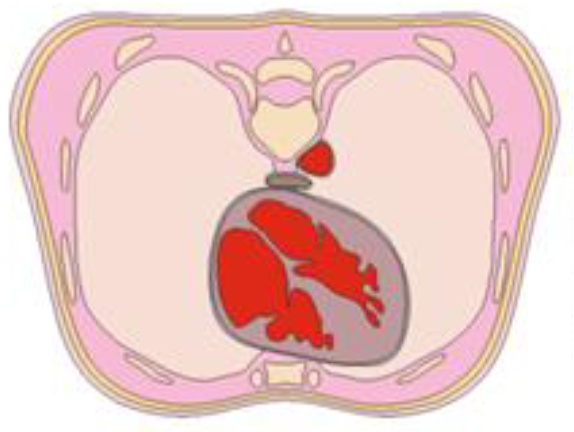
\includegraphics[width=0.5\textwidth]{./Figures/fig60}
	\caption{Modelo de tórax polifásico,}
	\label{fig:60}
\end{figure}

La resistividad disminuye a medida que los colores pasan de amarillo claro (que corresponde a huesos y cartílagos) al rojo (que corresponde a la sangre en los ventrículos cardíacos y en la aorta).

Algunas veces se pueden introducir simplificaciones adicionales, dependiendo del problema considerado.

Si lo que interesa son los campos en las cavidades del corazón, se puede sustituir el modelo más completo por un primer modelo más simple en el cual, además de las cavidades cardíacas, se tienen en cuenta dos fases homogéneas, una correspondiente a los pulmones y la otra al resto de los tejidos.

Simplificaciones sucesivas del modelo realizadas teniendo en cuenta el tipo de problema que se quiere estudiar. Por ejemplo en la figura \ref{fig:61}, el caso un problema relacionado con las cavidades del corazón. En esa figura las resistividades de cada fase aparecen en $\Omega m$. Cada una de las tres fases se caracteriza por la región que ocupa y por su conductividad.

\begin{figure}[H]
    \centering
    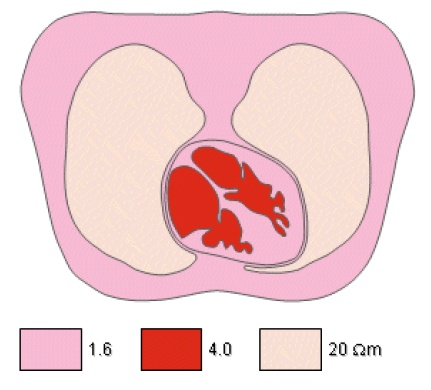
\includegraphics[width=0.5\textwidth]{./Figures/fig61}
	\caption{Modelo relacional con las cavidades del corazón}
	\label{fig:61}
\end{figure}

Un segundo modelo, aún más simplificado, se puede ver en corte de la figura \ref{fig:62}. Este modelo distingue solamente dos fases: una fase que representa a las cavidades cardíacas y otra fase que representa al resto de los tejidos.

\begin{figure}[H]
    \centering
    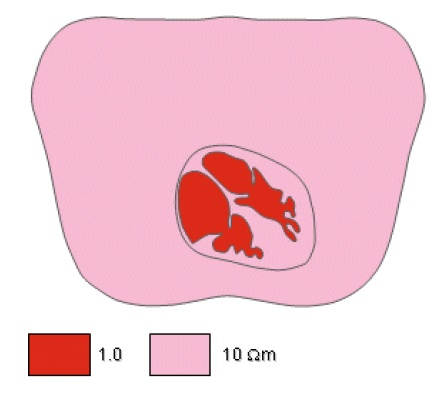
\includegraphics[width=0.5\textwidth]{./Figures/fig62}
	\caption{Modelo simplificado}
	\label{fig:62}
\end{figure}

Considerados globalmente, los tejidos biológicos y e incluso sus células, se comportan como medios diamagnéticos. Los eritrocitos desoxigenados son una excepción, pues se comportan como paramagnéticos. Además, en bacterias y tejidos biológicos de los animales y las plantas puede haber partículas ferrimagnéticas (formadas de magnetita).

La exposición a campos ambientales, a campos asociados a instalaciones industriales, a campos muy intensos en el diagnóstico médico (imágenes de resonancia magnética nuclear) y en el tratamiento médico (estimulación magnética funcional) es cada vez más frecuente. Esto ha aumentado el interés por los mecanismos de interacción de los campos con los tejidos biológicos y la preocupación por establecer umbrales de exposición que no deben ser superados.

En este capítulo el énfasis se pone en estudiar de algunos de los fenómenos que involucran el campo magnético en las estructuras y procesos correspondientes a los últimos dos niveles de la jerarquía. En ocasiones haremos referencia a resultados obtenidos en la investigación de los dos primeros niveles.

En particular consideraremos algunos de los fundamentos físicos de la interacción de los campos magnéticos ambientales con los organismos:

\begin{itemize}
	\item Orientación de partículas en campos magnéticos estáticos.
	
	\item Traslación de partículas en campos magnéticos no homogéneos.
	
	\item Aparición de fuerzas sobre partículas cargadas en movimiento en campos magnéticos.
	
	\item Inducción de corrientes eléctricas en el conductor de volumen de los tejidos debidas a variaciones del campo magnético en el tiempo o al movimiento de los organismos inmersos en campos magnéticos estáticos que presentan variaciones espaciales.

\end{itemize}

Para el caso de campos estáticos homogéneos, estudiamos brevemente la orientación y deformación de células y de estructuras supramoleculares debido a fuerzas y a torques magnéticos. En tejidos isótropos esas fuerzas de volumen (fuerzas de traslación) aparecen cuando la susceptibilidad magnética del tejido no es uniforme.

Los torques pueden actuar sobre las partículas de magnetitas mencionadas previamente. También aparecen torques en campos homogéneos debidos a anisotropías en la susceptibilidad magnética de estructuras supramoleculares diamagnéticas, como las membranas celulares y los cromosomas.

Para campos magnéticos estáticos no homogéneos, consideramos la aparición de fuerzas magnéticas y sus efectos.

Para campos dinámicos, revisamos la generación de corrientes eléctricas inducidas en el conductor de volumen de los tejidos, que cuando disipan energía siempre producen calor. Si poseen las características adecuadas esas corrientes inducidas pueden estimular a nervios, a músculos esqueléticos e inclusive al músculo cardíaco.

A diferencia del campo eléctrico, el campo magnético no es atenuado en la interfaz entre el aire (o el agua) y el organismo, debido a que las diferencias en las permeabilidades magnéticas de estos medios difieren muy poco entre sí, al igual que las diferencias en la permeabilidad que se encuentran entre diferentes tejidos.

Esto es así exceptuando las partículas ferri-magnéticas de dimensiones del orden de decenas de nanómetros o de micrómetros, que pueden aparecer en el interior de algunas bacterias y en tejidos de animales. Estas partículas pueden tener un rol fisiológico, o pueden ser el resultado de la contaminación de tejidos (pulmones, hígado) por inhalación o ingesta \footnote{Las partículas que poseen un rol fisiológico difieren desde el punto de vista cristalográfico de las partículas provenientes de la contaminación.}. 

Las mediciones de la susceptibilidad magnética del hígado y de los pulmones suministran indicadores del grado de esa contaminación. Ubicando el tórax de una persona, cuyos pulmones se han contaminado por inhalación de polvo con contenido ferrimagnético, en un campo magnético constante lo bastante intenso durante algunos segundos, las partículas de magnetita se orientan paralelamente al campo externo. Cuando éste desaparece, el campo residual debido a los momentos magnéticos sufre un proceso de relajación. La evolución del campo residual se puede medir y se obtiene lo que se denomina magneto-neumografía.

Este procedimiento suministra información sobre la contaminación en los alvéolos, sobre parámetros viscoelásticos celulares y sobre el movimiento de células del sistema inmunitario que capturan y eliminan material extraño al tejido.

Aunque las diferencias en la susceptibilidad magnética entre los diferentes tejidos diamagnéticos son mucho menores, la diferencia de susceptibilidad magnética entre el músculo cardíaco y la sangre en las cavidades ventriculares es suficiente para permitir la determinación de volúmenes.

El campo magnético puede actuar sobre momentos magnéticos a nivel nuclear (interacción empleada en los métodos basados en la resonancia magnética nuclear) y atómico (efecto Zeeman extrínseco), ya estudiados previamente en este libro. Además, el campo puede interactuar a niveles moleculares y supramoleculares, y sobre las corrientes eléctricas circulantes en los tejidos biológicos, relacionadas con algunos los procesos fisiológicos.

Si los procesos en un organismo se ven influidos por un campo magnético, puede ser considerado como un detector de ese campo. Si así se lo considera, un campo magnético externo podría pensarse como una señal. Para ser detectada, debe superar el nivel de ruido. Este es otro de los temas que abordaremos en lo que sigue.

También estudiamos los fundamentos físicos de la generación de campos magnéticos por esos mismos organismos y los fundamentos de la medición de esos campos mediante instrumentos externos, como el SQUID estudiado previamente en este libro en la parte dedicada a la superconductividad, incluyendo junturas Josephson.

En medicina el magneto-cardiograma, el magneto-encefalograma y la magneto-miografía suministran información complementaria a la obtenida respectivamente del electrocardiograma, el electroencefalograma y la electromiografía.

En general no es posible desvincular totalmente los campos eléctricos que aparecen en el conductor de volumen electrolítico formado por los tejidos biológicos, de los campos magnéticos ambientales o producidos por los organismos.

Se pueden distinguir dos fuentes principales de los campos magnéticos producidos por los organismos.

\begin{itemize}
	\item Una de estas fuentes son las corrientes eléctricas que acompañan a los procesos fisiológicos en el corazón, el sistema nervioso y los músculos, o menos frecuentemente y con menor importancia, las corrientes eléctricas asociadas al campo eléctrico generado cuando el organismo se mueve respecto de un campo magnético externo.
	
	\item La otra fuente del campo magnético producido en los organismos son los cuerpos magnetizados presentes en los tejidos biológicos o en el interior de las bacterias.
\end{itemize}

Cuando se tienen en cuenta las interacciones de los tejidos biológicos con campos externos variables con el tiempo, en condiciones casi-estacionarias (es decir, cuando se puede despreciar la corriente de desplazamiento en el interior de los tejidos) un campo magnético variable local induce un campo eléctrico local variable.

Pero el campo eléctrico variable por sí mismo (es decir, sin la intermediación de las corrientes eléctricas asociadas a esos campos) no genera un campo magnético en estas condiciones.
Pero a frecuencias lo bastante elevadas como para no poder despreciar la corriente de desplazamiento, el campo eléctrico local variable induce directamente un campo magnético local y se transforma entonces en una fuente de campo magnético.

Puesto que los seres humanos hemos estado expuestos durante eones a los campos eléctricos y magnéticos naturales, presenta interés revisar algunos aspectos relacionados con las amplitudes y frecuencias de estos campos para poder compararlos con los campos originados en las actividades propias de nuestra Era Tecnológica. Comenzaremos entonces por este tema.

\section{Campos geomagnéticos y geo-eléctricos estáticos}

En la superficie de nuestro planeta, las plantas, los animales y los seres humanos se encuentran con campos estáticos de inducción magnética $\V{B}$ de magnitudes comprendidas entre $33\mu T$ y $67 \mu T$ y campos eléctricos también estáticos $\V{E}$ con magnitudes en un entorno de los $100 V/m$, pudiendo alcanzar los $100 kV/m$ bajo una nube de tormenta. Estos campos estáticos no parecen estar implicados en efectos biológicos.

El campo geo-eléctrico estático no parece producirlos en ausencia de vías de descarga a tierra que permitan la instalación de corrientes eléctricas significativas en el conductor de volumen de los tejidos.

Pese a que en la mayor parte de los organismos el campo geomagnético estático no parece producir efectos biológicos en ausencia de campos oscilantes que se le superpongan, en algunos organismos el campo geomagnético estático se relaciona con la posibilidad de un cierto grado de orientación espacial.

\subsection{Orientación de bacterias en el campo magnético terrestre}

Algunas bacterias que viven en medios acuático (lagos o mares) y son anaerobias, poseen en su interior un dipolo magnético $\overrightarrow{m}$ en forma de barra de varios micrómetros de longitud formada por pequeños cuerpos (magnetosomas) de decenas o centenares de nanómetros, magnetizados y adheridos entre sí, con la misma orientación de su momento magnético. ver figura \ref{fig:magnetosoma01}
Los magnetosomas están formados por una partícula de magnetita (ferrimagnética)\footnote{En biología y medicina a menudo se hace referencia a ellos como si fueran ferromagnéticos.} rodeada por una membrana. Cada partícula constituye por sí misma un único dominio magnético.


\begin{figure}[H]
    \centering
    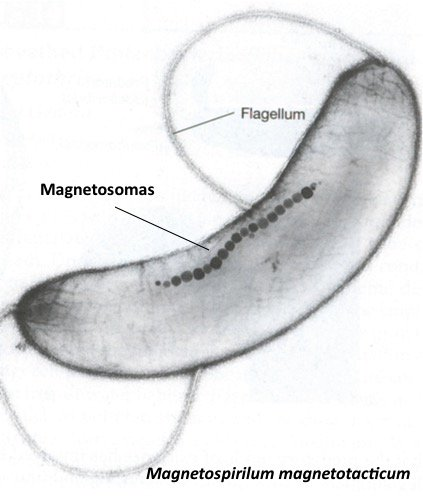
\includegraphics[width=0.5\textwidth]{./Figures/magnetosoma01}
	\caption{Bacteria procarionte con magnetosoma}
	\label{fig:magnetosoma01}
\end{figure}

El campo magnético terrestre produce un torque $\tau_{m}=\overrightarrow{m} \times \overrightarrow{B_{T}}$ sobre ese dipolo. 
Este torque gira la bacteria tendiendo a alinearla con el campo magnético terrestre.

La bacteria alineada con el campo se desplaza activamente utilizando sus cilias o su flagelo\footnote{El movimiento en sí resulta de la actividad de la bacteria, pero la orientación en el campo magnético externo es puramente pasiva.}. 

Si la magnetización de la barra de magnetosomas es la apropiada, el microorganismo se aleja de la superficie rica en oxígeno (donde no puede vivir) y se dirige a las regiones profundas, pobres en oxígeno, donde puede vivir y reproducirse.

Cuando una de estas bacterias se reproduce, la mitad de la barra de magnetosomas pasa cada célula bacteriana hija.

Estas sintetizan nuevos magnetosomas que se añaden a los recibidos de la célula bacteriana madre hasta que las longitudes de las barras alcancen valores que aseguren torques adecuados para girar la célula bacteriana en el campo magnético terrestre.


En la figura \ref{fig:63} vemos el esbozo de algunas líneas del campo magnético de la Tierra. Se ve la inclinación del campo magnético en dos localidades. En la figura se puede apreciar la descomposición del campo en dos: una componente vertical (que es máxima en las cercanías de los polos y mínima en las proximidades del ecuador) y una componente horizontal (que es máxima en las proximidades del ecuador y mínima en las cercanías de los polos). La descomposición corresponde a dos localidades señaladas con círculos en la superficie terrestre.

\begin{figure}[H]
    \centering
    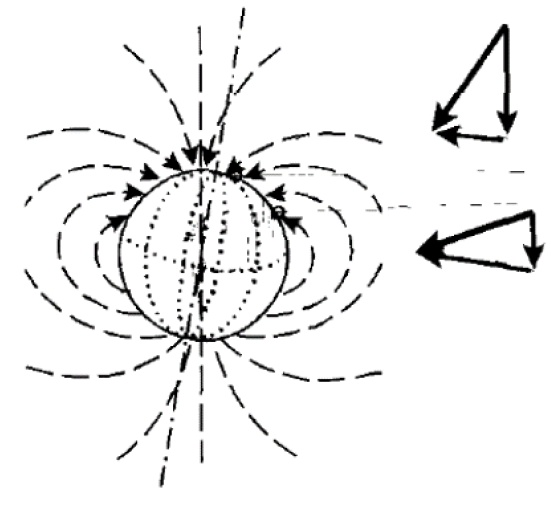
\includegraphics[width=0.5\textwidth]{./Figures/fig63}
	\caption{Esbozo del campo magnético terrestre}
	\label{fig:63}
\end{figure}

Desde hace mucho tiempo se dispone de evidencia acerca de la orientación magnética de animales (insectos, aves, peces y mamíferos) mediante diversos tipos de receptores geomagnéticos, pero todavía no hay suficiente consenso entre los investigadores acerca de los mecanismos involucrados en cada caso.

\section{Campos geomagnéticos y geo-eléctricos variables}

Como los campos geo-eléctricos y geomagnéticos presentan fluctuaciones asociadas a las tormentas atmosféricas y a las perturbaciones en las cargas de la ionósfera, todos los organismos biológicos se encuentran inmersos en campos variables que se superponen a los campos estáticos.
En el caso del campo eléctrico, aparecen fluctuaciones naturales de $0,01 V/m$ a frecuencias hasta de $10 Hz$.
Esas fluctuaciones decrecen hasta alcanzar valores cien veces menores, comprendidos entre $0,1$ y $0,6 mV/m$ a frecuencias de $50 Hz$.
A frecuencias mayores a algunos centenares de $Hz$ la amplitud de oscilación del campo eléctrico, superpuesta a su valor estático, es aún menor.

\subsection{Comparación con los campos generados por las líneas de transmisión de potencia}

Resulta interesante comparar estas amplitudes naturales de oscilación del campo eléctrico a $50 Hz$ con las amplitudes del campo eléctrico oscilante a esa misma frecuencia debajo de una línea de transmisión de potencia trifásica, que puede alcanzar unas decenas de $kV/m$ y son capaces de encender un tubo fluorescente que resplandece sin alambres de conexión cuando se lo mantiene en el aire debajo de la línea. La relación de amplitudes es de $1$ a $10^{7}$.

En el caso del campo geomagnético, las amplitudes de las oscilaciones a $1 Hz$ son de $1 nT$, mientras que a frecuencias comprendidas entre $10 Hz$ y $100 Hz$ dichas amplitudes son de $10 pT$.
Si bien durante una tormenta magnética la intensidad puede aumentar en $0,5 \mu T$, este aumento se produce en minutos u horas.
Debido a las influencias del sol y de la luna sobre las corrientes iónicas en la alta atmósfera, aparecen variaciones diurnas, con amplitudes de aproximadamente $30 nT$.

Además, superpuestos a esos campos lentamente variables asociados a eventos atmosféricos irregulares, aparecen otros campos, débiles, generados por un fenómeno de resonancia en la cavidad comprendida entre la superficie terrestre y la capa más baja de la ionósfera. La energía de estos campos proviene de la descarga de rayos.

La formación de campos periódicos con frecuencias de aproximadamente $8 Hz$, $14,1 Hz$, $20,3 Hz$ y $32,5 Hz$ se debe a los fenómenos de propagación y reflexión en esa cavidad resonante. Este fenómeno se conoce como \textbf{Resonancia de Schumann}.
Las amplitudes de las distintas componentes disminuyen al aumentar la frecuencia, pero en general aún las más bajas no superan los $20 nT$ (generalmente son bastante menores).
Es un hecho interesante la variación en las frecuencias de Schumann provocadas por modificaciones en el espesor de la cavidad resonante. Ese espesor se modifica debido los efectos gravitacionales del sol, la luna y de algunos planetas sobre la ionósfera.

Resulta asimismo interesante comparar la amplitud de oscilación de $10 pT$ del campo magnético a $50 Hz$ con los más de $0,1 \mu T$ de amplitud de oscilación a esa misma frecuencia, que se pueden medir debajo de algunas líneas de transmisión de potencia. La relación de amplitudes es de $1$ a $10^{4}$.

En relación con estas comparaciones, es conveniente llamar la atención sobre el apantallamiento que sufren los campos eléctricos ambientales, naturales y artificiales, por árboles, edificios y otros objetos.
Ese apantallamiento en general no se manifiesta en el caso del campo magnético ambiental, natural o artificial, que disminuye fundamentalmente cuando aumenta la distancia entre su fuente y el punto de observación.
Por otra parte, el campo eléctrico en un cierto punto situado debajo de una línea de transmisión de potencia depende del voltaje con el cual se transporta la energía, cuya amplitud es constante. En cambio, el campo magnético en ese mismo punto varía cuando la corriente que circula por la línea se modifica durante el curso de un día.

Como los campos eléctricos y magnéticos artificiales son mucho mayores que los campos naturales que oscilan a esas mismas frecuencias y que nos han acompañado durante nuestra evolución biológica como especie, parece que debiera ser de interés el estudio de sus posibles efectos sobre nuestro organismo.

\subsection{Ruidos, campos y contaminaciones}

La mayor parte de las personas que investigan los efectos biológicos de los campos electromagnéticos asume que los campos y corrientes asociados con el funcionamiento normal del organismo no deben producir ellos mismos (ni deben actuar como promotores de) daños significativos a nivel de las células, ni sobre sus orgánulos funcionales ni sobre el ADN.
Entonces parece que no se deberían esperar efectos perjudiciales provocados por las fluctuaciones aleatorias naturales de los campos eléctricos y magnéticos a nivel de las membranas celulares.
Lo mismo cabe esperar en el caso de los campos magnéticos generados por las corrientes eléctricas que normalmente circulan por el organismo, asociadas a las actividades del sistema nervioso central, del sistema neuromuscular y del corazón.

Como dijimos en la introducción a este capítulo, si un organismo se ve afectado de cualquier manera por un campo externo, parece que se lo podría considerar como un detector natural para ese campo.

El campo externo sería una señal que recibe el detector, señal que para ser detectada debe superar al ruido.

Suponiendo que esto sea así, la intensidad de estos campos de ruido suministra una escala natural para comparar las intensidades de los campos intracelulares o en el interior de las membranas, generados por la exposición del organismo a campos externos.
Si las intensidades de estos últimos campos son mucho menores o a lo sumo del mismo orden de magnitud que los campos de ruido, parecería que no deberían producir efectos significativos.

Los magnetosomas pueden resultar de importancia en relación con posibles efectos sobre las estructuras supramoleculares de las células, debidos a un campo magnético externo.
En 1992, Kirschvink y otros informaron que el cerebro humano contiene varios millones de micropartículas ferrimagnéticas por gramo de tejido: los magnetosomas que ya mencionamos a propósito de la orientación de algunas bacterias en el campo magnético de la Tierra.
En 1995, Kobayashi y otros descubrieron que la contaminación con magnetosomas puede afectar los experimentos bioeléctricos y biomagnéticos realizados con cultivos de tejidos cuyas células normalmente no contienen magnetosomas.

Esta contaminación puede deberse a los materiales plásticos previamente esterilizados que se utilizan en experimentos de laboratorio con cultivos de tejidos: contienen partículas ferrimagnéticas de menos de 100 nm, que son incorporadas fácilmente por las células de la serie blanca de la sangre.

Para estimar el cociente señal-ruido para uno de estos pequeños magnetosomas en un campo magnético estático, se puede asumir una situación de equilibrio local, como se hace en la termodinámica de procesos irreversibles.

Esta suposición puede hacerse para la mayor parte de las redes de reacciones bioquímicas y procesos de transporte en el interior celular y en las membranas biológicas, aunque no en todos los casos. En particular, puede que no sea posible hacer esta suposición durante algunas de las bruscas transiciones de fase fuera del equilibrio que se producen a nivel celular.

Admitiendo equilibrio local y la posibilidad de una descripción aplicando la física estadística clásica, la densidad de probabilidad $f_{m}(\Theta)$ correspondiente al ángulo $\theta$ que el momento magnético $\overrightarrow{m}$ de un magnetosoma forma con el campo magnético terrestre $\overrightarrow{B_{T}}$ viene dada por:

\begin{equation}
	\label{eq:60}
	f_{m}(\theta)=\dfrac { 2\pi e^{\left( \dfrac{m B_{T} Cos(\theta)}{k_{B}T}\right) }}{4\pi \left( \dfrac{k_{B}T}{m B_{T}} \right) Sinh\left( \dfrac{ m B_{T}}{k_{B}T} \right)}    
\end{equation}

La expresión de la ecuación \ref{eq:60} es formalmente la misma que se aplicó originalmente en un análisis microscópico del paramagnetismo basado en la física estadística clásica (Sommerfeld, 1956). Ahora la estamos aplicando en un análisis a nivel mesoscópico.

En ausencia de campo externo el factor de Boltzmann ${e^{\left( \dfrac{m B_{T} Cos(\theta)}{k_{B}T}\right)}}$ se reduce a la unidad para todos los ángulos posibles y la densidad de probabilidad de que el momento magnético forme un ángulo $\theta$ con el campo se reduce a $\dfrac{1}{4\pi} 2 \pi Sin(\theta) = \dfrac{1}{4\pi}\dfrac{d\Omega}{d\theta}$ donde ${\dfrac{d\Omega}{d\theta} = 2\pi Sin(\theta)}$. Aquí $d\Omega=2\pi Sin(\theta) d\theta$ es un elemento de ángulo sólido y $4\pi$ es el ángulo sólido total, de modo que $\dfrac{d\Omega}{4\pi}$ es la probabilidad de que, en ausencia de campo externo, el ángulo entre el momento magnético y el campo se encuentre entre $\theta$ y $\theta + d\theta$.

En la figura \ref{fig:64} se puede ver un elemento de ángulo sólido correspondiente al caso en el que las velocidades de desplazamiento de la bacteria forman un ángulo $\theta$ con la dirección y sentido del campo magnético. El eje vertical corresponde a la dirección del campo magnético externo. La banda rayada representa el elemento de ángulo sólido $d\Omega=2\pi Sin(\theta) d\theta$ Sobre esa banda se muestra un vector de momento magnético.


\begin{figure}[H]
    \centering
    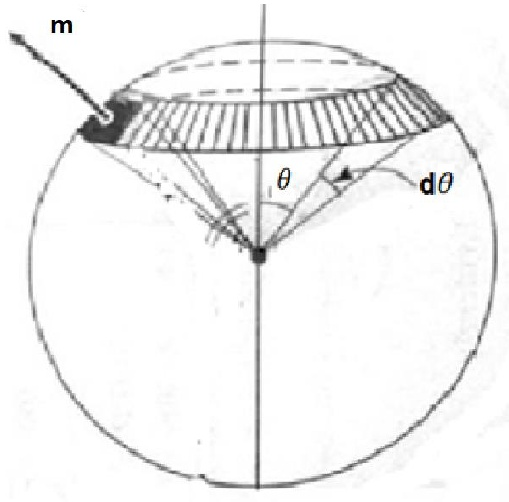
\includegraphics[width=0.5\textwidth]{./Figures/fig64}
	\caption{Sección de ángulo sólido}
	\label{fig:64}
\end{figure}

La componente del momento magnético del magnetosoma paralela al campo es $m\, Cos(\theta)$. El promedio de esta componente paralela al campo viene dado por la fórmula\footnote{Utilizamos una barra por encima de la magnitud que se promedia $\bar{ }$ para indicar un promedio tomado en el sentido de la física estadística. El símbolo $<\;,\;>$ se reserva para ser utilizado en desarrollos que involucran mecánica cuántica.}

\begin{equation}
	\label{eq:61}
	m_{\vert\vert}=\overline{m\, Cos(\theta)}=\int_{0}^{\pi}f_{m}(\theta)(m\,Cos(\theta))d\theta=m\left[ Ctgh\left( \dfrac{m B_{T}}{k_{B}T}\right) -\dfrac{k_{B}T}{m\,B_{T}} \right] 
\end{equation}


La función $\mathcal{L}(x)=Ctgh(x)-\dfrac{1}{x}$ fue introducida por Langevin\footnote{Langevin obtuvo la función $\mathcal{L}(x)$ en una investigación, empleando herramientas de física estadística clásica, de las propiedades dieléctricas de un gas ideal, cuyas moléculas poseen momentos dipolares permanentes, en un campo externo. Posteriormente extendió este enfoque al paramagnetismo (Sommerfeld, 1956).}. Si $x$ es pequeño respecto de la unidad o a lo sumo $x\lesssim 1$ , $\mathcal{L}(x)$ se comporta como $\dfrac{1}{3}x$ mientras que si es grande respecto de la unidad $\mathcal{L}(x)$  se encuentra muy próxima a $1$, comportándose como $1-\dfrac{1}{x}$.

Así, cuando $x=10$ la función de Langevin toma un valor próximo a $0,9$, de modo que la dirección del momento magnético se encuentra en promedio muy cercana a la dirección del campo externo.

El campo magnético tiende a alinear mientras que las interacciones térmicas con las partículas del medio tienden a desalinear el momento magnético del magnetosoma. En consecuencia, el número no-dimensionado $x=\dfrac{mB}{k_{B}T}$ se puede interpretar como una medida del cociente señal magnética/ruido térmico, donde $mB$ es la energía máxima de interacción magnética entre la partícula magnetizada y el campo magnético externo y $k_{B}T$ es una estimación de la energía del ruido térmico local. Cuando ese número posee un orden de magnitud de la unidad o menor, el ruido térmico tiende a romper la alineación del momento magnético con el campo externo y prepondera el desorden molecular sobre el orden asociado a la alineación.

Por el contrario, cuando $\dfrac{mB}{k_{B}T}$ es de un orden superior a la unidad, la señal supera al ruido y la alineación se puede estabilizar, aunque con fluctuaciones tanto más frecuentes cuanto menor sea el orden numérico del número no-dimensionado.

Supongamos que un magnetosoma se encuentra en un campo magnético terrestre de $5.10^{-5} T$, actuando a una temperatura local de $300^{o}K$.
En general las partículas magnéticas que no se deben a la contaminación y parecen cumplir un rol fisiológico poseen un diámetro próximo a los $50 nm$, alcanzando algunas veces los $100 nm$. Si su diámetro es demasiado grande, se podrían formar varios dominios con diferentes orientaciones magnéticas. En ese caso el momento magnético se vería disminuido respecto del caso en el cual un único dominio abarca la totalidad de la partícula. Si su diámetro es demasiado pequeño, las fluctuaciones térmicas en el medio podrían destruir el alineamiento del momento magnético de la partícula con el campo externo.

Si el diámetro de un magnetosoma es de $50 nm$ cabe esperar un momento magnético de $6,4.10^{-17} Am^{2}$ y en este caso $\dfrac{mB}{k_{B}T}$ adopta como valor $0,77$. Si su diámetro es de $100 nm$ y está magnetizado formando un dominio único, su momento magnético es de $2.10^{-15} Am^{2}$ y ahora $\dfrac{mB}{k_{B}T}$ vale $24$.


Para magnetosomas con diámetros crecientes entre los $50 nm$ y los $100 nm$, el número $\dfrac{mB}{k_{B}T}$ toma todos los valores intermedios entre $0,77$ y $24$. Así pues, debido a que puede dar lugar a una elevada relación señal-ruido en el campo magnético terrestre o en campos externos más intensos, la existencia de magnetosomas, integrados en estructuras supramoleculares y eventualmente actuando en forma sinérgica, podría tener como consecuencia la aparición de algún efecto biológico, como la apertura de canales iónicos en las membranas celulares.

\section{Modelo simplificado de efecto fisiológico del campo magnético}

Consideremos un modelo de apertura de poros en una membrana biológica, asociada a la rotación de un magnetosoma esférico de radio\footnote{El radio $a$ se debe expresar en m.} $a$ y de momento magnético $m=2.10^{6} a^{3} Am^{2}$, en un campo magnético variable que se superpone al campo magnético terrestre.

Supongamos que el magnetosoma se halla integrado en la membrana, adherido a la compuerta de un canal iónico.

Además, supongamos que cuando el magnetosoma se encuentra en su posición de equilibrio alineado con el campo magnético terrestre, una compuerta, también en su posición de equilibrio, obtura el canal.

Se añade un campo externo que varía con el tiempo $B_{p}(t)$ perpendicular al campo magnético terrestre $B_{T}$ (que se considera constante) que tiende a rotar al magnetosoma en el plano determinado por ambos campos, un cierto ángulo $\theta(t)$ respecto de su posición de equilibrio alineado con $B_{T}$ .

Cuando el magnetosoma rota arrastra tras de sí a la compuerta que rota a su vez un mismo ángulo $\theta(t)$ y como consecuencia el canal se abre.

Cuando la apertura alcanza un umbral $\theta_{u}$, se desencadena un proceso regenerativo que permite que un pulso de corriente de iones de cierto tipo atraviese la membrana.

A medida que la compuerta se aleja de su posición de equilibrio, aparece un torque $\tau_{c}(\theta)$ que se opone a la apertura.

Para los fines de construir un modelo matemático simple asumiremos que lo podemos linealizar introduciendo una constante elástica $k_{c}$: $\tau_{c}=-k_{c}\theta$.

A este torque se le suma un torque restaurador debido al campo magnético terrestre $\tau_{T}=-mB_{T}Sin(\theta)$, un torque perturbador $\tau_{p}=mB_{p}(t)Cops(\theta)$, debido al campo externo perturbador, un torque $\tau_{R}(t)$ relacionado con el ruido térmico y un torque restaurador $\tau_{v}=-\alpha\dT{\theta}{t}$ debido a fuerzas viscosas.

Si la viscosidad del medio es $\mu$ resulta: $\alpha=8\pi\mu a^{3}$

Los valores medidos para $8\pi\mu$ se ubican generalmente entre $0,003$ y $0,015 Ns/m^{2}$ lo que sugiere tomar como valor representativo, para $\mu=0,0035 Ns/m^{2}$: $\alpha=0,009 a^{3}$
El momento de inercia $I$ respecto del eje de rotación que pasa por el centro de la esfera, suponiendo que el material ferrimagnético posee una densidad uniforme\footnote{La magnetita ($Fe_{3}O_{4}$) posee una densidad de $5240 kg/m^{3}$} $\rho$ viene dado por: $I=\dfrac{8}{15}\pi\rho a^{5}$. Entonces la ecuación del movimiento de rotación del magnetosoma adherido a la compuerta de un canal que atraviesa la membrana celular se puede escribir así:

\begin{equation}
	\label{eq:62}
	I\dfrac{d^{2}\theta}{dt^{2}}=-\alpha\dfrac{d\theta}{dt}-k_{c}\theta-mB_{T}Sin(\theta)+mB_{p}(t)Cos(\theta)+\tau_{R}(t)
\end{equation}

Para concretar, consideremos que el campo externo oscila con una frecuencia angular $\omega$ y una amplitud $B_{p}$: $B_{p}=B_{0}Cos(\omega t)$. Para simplificar el modelo, en una primera aproximación no tomaremos en cuenta el torque de ruido $\tau_{R}(t)$, aproximaremos $Sin(\theta= \approx \theta$ y $Cos(\theta) \approx 1$.

Si el número sin dimensiones\footnote{Este número se obtiene sustituyendo una solución armónica de frecuencia angular $\omega$ en el término inercial $I\dfrac{d^{2}\theta}{dt^{2}}$ y en el término disipativo $\alpha\dfrac{d\theta}{dt}$ , dividiendo luego la amplitud del resultado obtenido para el término inercial por la amplitud del resultado obtenido para el término disipativo} $\dfrac{\omega I}{\alpha}=\left( \dfrac{\rho}{\mu}\right)\dfrac{\omega a^{2}}{15}\ll1 1 $, el torque viscoso es lo bastante intenso como para no tener en cuenta en la ecuación el término debido a la aceleración angular.

Como para una partícula de magnetita de $50 nm$ de densidad $5240 kg/m^{3}$ inmersa en un medio con una viscosidad $\mu=0,0035 Ns/m^{2}$, $\left( \dfrac{\rho}{\mu}\right)\dfrac{\omega a^{2}}{15}$ es del orden de $10^{−10}\omega$, y como las frecuencias angulares de los campos oscilantes considerados son de un orden numérico inferior a $10^{6}$ Hz, en lo que sigue asumiremos el dominio de la disipación sobre la inercia.

En ese caso la ecuación del movimiento se reduce a:

\begin{equation}
	\label{eq:63}
	\dfrac{d\theta}{dt}+\dfrac{k_{c}+mB_{T}}{\alpha}\,\theta=\dfrac{mB_{0}}{\alpha}Cos(\omega t)
\end{equation}

La solución estacionaria de esta última ecuación es: $\theta(t)=\theta_{m}Cos(\omega t - \varphi(\omega))$ con:

\begin{equation*}
	\label{eq:64}
	tg\left(\varphi(\omega) \right) = \dfrac{\alpha\omega}{k_{c}+mB_{T}}
	=\dfrac{\omega}{\left( \dfrac{k_{c}}{\alpha}\right) +\left( \dfrac{m}{\alpha}\right) B_{T}}
\end{equation*}

y

\begin{equation*}
	\label{eq:65}
	\theta_{m} = \dfrac{mB_{0}}{\sqrt{\alpha^{2}\omega^{2}(k_{c}+mB_{T})^{2}}}
	=\dfrac{B_{0}}{\sqrt{\left( \dfrac{\alpha}{m}\right) ^{2}\omega^{2}+\left( \dfrac{k_{c}}{m}+B_{T}\right) ^{2}}}
\end{equation*}

Como tanto $\alpha$ como $m$ son proporcionales a $a^{3}$, $\dfrac{\alpha}{m}$ resulta independiente del radio del magnetosoma.

Cuando $\theta_{m}>\theta_{u}$ la compuerta rota, alcanza y supera el umbral. El pulso iónico a través del canal se produce: el campo magnético externo habrá dado lugar a un efecto biológico.


\subsection{Influencia de las fluctuaciones estadísticas sobre la orientación de partículas magnetizadas}


Supongamos que el campo $B_{p}(t)$ desaparece y una partícula magnetizada permanece en el campo magnético de la tierra.

En equilibrio local se puede aplicar la distribución de Boltzmann para una energía de interacción $U(\theta)= -mB_{T}Cos(\theta)$ con $0\leq\theta\leq\pi$.

Para ángulos lo bastante pequeños, si aproximamos $Cos(\theta)$ por la fórmula aproximada $1-\dfrac{1}{2}\theta^{2}$ obtenemos la aproximación $U(\theta)\approx -mB_{T} + \dfrac{mB_{T}}{2}\theta^{2}$.

Si admitimos trabajar con esta última expresión de la energía potencial sin limitaciones, se puede aplicar el teorema de equipartición de la energía de la física estadística para obtener el valor medio cuadrático $\theta_{mc}$ del ángulo entre el momento magnético y el campo en un medio de temperatura local $T$ :

\begin{equation}
	\label{eq:66}
	\theta_{mc} =\sqrt{\overline{\theta^{2}}} = \dfrac{k_{B}T}{mB_{T}}
\end{equation}

Asumiendo un momento magnético $m=2.10^{6} a^{3} Am^{2}$ y un campo terrestre de magnitud $B_{T}=5.10^{−5} T$ resulta: $\theta_{mc}=\dfrac{k_{B}T}{100a^{3}}$

Esta expresión del valor medio cuadrático del ángulo entre $\V{m}$ y $\overrightarrow{B_{T}}$ disminuye como el recíproco del cubo del diámetro de la partícula.
La razón por la cual $\theta_{mc}$ no está acotado superiormente cuando el diámetro tiende a cero es la validez de la aproximación $Cos(\theta)\approx 1-\dfrac{1}{2}\theta^{2}$ que permitió aplicar el teorema de equipartición de la energía. Solo si $\theta$ es lo bastante pequeño la aproximación resulta aceptable.

Para un magnetosoma ligado a la compuerta de un canal iónico, la energía potencial en el campo magnético terrestre se puede aproximar así, añadiendo la energía potencial elástica de la compuerta rotada: 

\begin{equation}
	\label{eq:67}
U(\theta)\approx -mB_{T} + \dfrac{mB_{T}}{2}\theta^{2}+\dfrac{k_{c}}{2}\theta^{2}
\end{equation}

Entonces: 

\begin{equation}
	\label{eq:68}
		\theta_{mc} =\sqrt{\overline{\theta^{2}}} = \dfrac{k_{B}T}{k_{c}+mB_{T}}
\end{equation}

Asumiendo nuevamente un momento magnético $m=2.10^{6} a^{3} Am^{2}$ y un campo terrestre de magnitud $B_{T}=5.10^{−5} T$ resulta:

\begin{equation}
	\label{eq:69}
		\theta_{mc} = \dfrac{k_{B}T}{k_{c}+100a^{3}}
\end{equation}


También para este se utilizó la aproximación $Cos(\theta)\approx 1-\dfrac{1}{2}\theta^{2}$ con las limitaciones que conlleva.

Cuando es superado el umbral de rotación $\theta_{u}$, se desencadena la apertura del canal. Si ${f_{m}}^{c}(\theta)$ es la densidad de probabilidad de que el momento magnético, ligado a la compuerta, en presencia del campo geomagnético, rote un ángulo $\theta$ debido a una fluctuación aleatoria, la probabilidad de apertura espontánea del canal viene dada por: $\int_{\theta_{u}}^{\pi}{f_{m}}^{c}(\theta)d\theta$.

Si se efectúa la aproximación $Cos(\theta)\approx 1-\dfrac{1}{2}\theta^{2}$ se puede utilizar, en lugar de ${f_{m}}^{c}(\theta)$, una distribución de Boltzmann, basada en el factor exponencial: 

$e^{-\left( \dfrac{k_{c} + mB_{T}}{2K_{B}T}\theta^{2} \right) }$. La integral se toma en ese caso entre $\theta_{u}$ y $+\infty$ .


\subsection{Aplicaciones de las fuerzas de traslación debidas a campos magnéticos no homogéneos a la separación de células}

Cuando una partícula magnetizada se encuentra en un campo de inducción magnética que, para un mismo instante de tiempo, varía de un punto a otro del espacio, sufre una fuerza de traslación\ref{eq:FPartMag}\citep{Kompaneyets}\citep{Landau8}.

\begin{equation}
	\label{eq:610}
	\V{F_{m}}=(\V{m}\cdot\nabla)\V{B}
\end{equation}

Esta expresión se reduce a $\V{F_{m}}=\nabla(\V{m}\cdot\V{B})$ cuando el momento magnético es intrínseco.

Cuando el medio es isotrópico y lineal: $\V{F_{m}}=\nabla(\frac{1}{2}m\cdot B)$

Una aplicación interesante de las fuerzas de traslación en campos no homogéneos es la separación magnética de células, utilizando partículas super-paramagnéticas (partículas paramagnéticas cuya susceptibilidad magnética relativa \ref{relMH} alcanza valores muy grandes respecto de 1 y se comportan en forma lineal en un campo externo).

Esas partículas exhiben sus propiedades magnéticas solo cuando se instala un campo magnético.
Se fijan partículas super-paramagnéticas de unos $50 nm$ de diámetro en puntos adecuados de un anticuerpo.

Este anticuerpo es capaz de unirse en forma específica al tipo de célula que interesa separar.
Con este procedimiento se pueden adherir un hasta centenar de partículas a cada célula.
Se pone la muestra en un campo magnético no homogéneo del orden de $1 T$ con un gradiente del orden de $10 T/m$.

Las células que interesan poseen, adheridas a su superficie, combinaciones de anticuerpos con partículas super-paramagnéticas, debido a lo cual se pueden separar de las otras células.

Otra aplicación de los campos no homogéneos es la entrega de fármacos ligados a micro-transportadores magnéticos en ciertos sitios del organismo.

La agitación magnética se emplea para modular la liberación de macromoléculas, contenidas en el espacio de poros de partículas de polímero que poseen inclusiones magnetizadas.

\subsection{Torques originados en anisotropías en las propiedades diamagnéticas de las estructuras moleculares y supramoleculares y Fuerzas de traslación asociadas a variaciones espaciales de la susceptibilidad magnética}


Cuando los materiales biológicos diamagnéticos y anisótropos, como la fibrina y el colágeno, o las membranas y los cromosomas, se exponen a campos magnéticos homogéneos, sufren un torque que tiende a rotarlos hacia la dirección determinada por sus propiedades de anisotropía. También se observa este fenómeno en moléculas de sustancias diamagnéticas, como el benceno.

Cuando en un material isótropo la susceptibilidad magnética varía de un punto a otro del medio, un campo magnético homogéneo produce una fuerza de traslación proporcional y paralela al gradiente espacial de esa susceptibilidad.

Consideremos un volumen mesoscópico $V_{0}$ de un material biológico diamagnético.
Como el tensor de susceptibilidad es simétrico, podemos orientar el sistema de ejes de coordenadas local según las direcciones principales de ese tensor.

La matriz que lo representa resulta diagonal.

Los elementos sobre la diagonal son las susceptibilidades principales $\chi_{1}$, $\chi_{2}$ y $\chi_{3}$, todas ellas números reales negativos.

En ese caso la matriz mencionada se puede escribir así: 

\begin{equation}
	\label{eq:611}
	\chi_{i,j} = 
	\begin{pmatrix}
	\chi_{1}  & 0       & 0       \\
	0         &\chi_{1} & 0       \\
	0         & 0       & \chi_{3} 
	\end{pmatrix}
\end{equation}

El aporte a la densidad de energía libre de Gibbs \ref{eq:D20} local, debida a procesos magnéticos, cuando el campo crece a partir de cero a temperatura y presión constantes se puede expresar, en ausencia de fenómenos de histéresis, por

\begin{equation}
	\label{eq:612}
	G = -\int_{0}^{\V{H}}\V{B}\cdot d \V{H}=
	-\dfrac{1}{2}\mu_{0}H^{2}-\mu_{0}\int_{0}^{\V{H}}\V{M} \cdot d \V{H}
\end{equation}

El segundo término del miembro de la derecha de esta ecuación se puede interpretar como el aporte debido a la magnetización local del material\footnote{Guggenheim, 1967}.

La magnetización se expresa como función lineal del campo $\V{H}$: $\V{M}= \bar{\bar{\chi}} \cdot \V{H}$

A partir de esta aproximación se obtiene para la densidad de energía libre:

\begin{equation}
	\label{eq:613}
	G_{M,H} = -\mu_{0}\int_{0}^{\V{H}}\V{M} \cdot d \V{H}= \dfrac{1}{2}\mu_{0}\V{H}\cdot \bar{\bar{\chi}} \cdot \V{H}
\end{equation}

Si las componentes del campo de excitación $\V{H}$ en dirección de los ejes principales del tensor son $H_{1}$, $H_{2}$ y $H_{3}$ resulta:

\begin{equation}
	\label{eq:614}
	G_{M,H} = -\dfrac{1}{2}\mu_{0}(\chi_{1}H_{1}^{2}+\chi_{2}H_{2}^{2}+\chi_{3}H_{3}^{2})
\end{equation}

Supongamos, además, que las susceptibilidades principales toman dos valores:
\begin{equation}
	\label{eq:615}
	\chi_{1}= \chi_{\vert\vert} \quad \text{y} \quad \chi_{2}=\chi_{3}=\chi_{\perp}
\end{equation}

Ambas susceptibilidades $\chi_{\parallel}$ y $\chi_{\perp}$ son negativas, pero asumiremos que 
$\vert \chi_{\parallel} \vert > \vert \chi_{\perp} \vert$

Si $H$ es la magnitud del campo externo, $\theta$ es el ángulo que forma $\V{H}$ con la primera dirección principal y $\varphi$ es el ángulo que forma la proyección $H_{\perp}$ de $\V{H}$ (sobre el plano determinado por las otras dos) con la segunda dirección principal:

\begin{equation}
\begin{aligned}
	\label{eq:616}
	H_{1} &= HCos(\theta)= H_{\parallel},\\
	H_{2} &= HSin(\theta)Cos(\varphi) = H_{\perp}Cos(\varphi),\\
	H_{3} & =HSin(\theta)Sin(\varphi) = H_{\perp}Sin(\varphi)
\end{aligned}
\end{equation}

La parte dependiente de la magnetización de la densidad de energía libre queda en este caso: 

\begin{equation}
	\label{eq:617}
G_{M, H}= -\dfrac{1}{2}\mu_{0}(\chi_{\parallel}Cos^{2}(\theta)+\chi_{\perp}Sin^{2}(\theta))B^{2}=-\dfrac{1}{2}\mu_{0}H^{2}(\chi_{\perp}+(\chi_{\parallel}-\chi_{\perp})Cos^{2}(\theta))
\end{equation}

El torque por unidad de volumen que actúa sobre el elemento de material biológico puede estimarse por la derivada parcial de $G_{M, H}$ respecto del ángulo, a igualdad de las demás variables (temperatura, presión).

Entonces el torque sobre la masa de estructura mesoscópica de volumen $V_{0}$ se puede calcular mediante la fórmula:

\begin{equation}
	\label{eq:618}
\tau_{m}=-\dfrac{1}{2}\mu_{0}H^{2}V_{0}\Delta\chi Sin(2\theta)
\end{equation}

En esta última fórmula $\Delta\chi=\chi_{\perp}-\chi_{\parallel}=\vert \chi_{\parallel} \vert - \vert \chi_{\perp} \vert > 0$

Ese torque por unidad de volumen tiende a rotar la estructura de modo que la dirección principal correspondiente a susceptibilidad de mayor valor absoluto se aproxime a la dirección del campo externo.

Lo que acontezca en definitiva y por tanto los posibles efectos biológicos del campo homogéneo, depende de la relación de fuerzas entre las que producen el torque debido al diamagnetismo anisótropo y las demás fuerzas actuantes en la superficie y el volumen del elemento mesoscópico de material considerado.

En estructuras con un grado elevado de anisotropía diamagnética y valores absolutos de los coeficientes de susceptibilidad también elevados, con un anclaje no muy fuerte a las estructuras vecinas, como por lo general es el caso de los cromosomas en el núcleo celular, se puede observar orientaciones inducidas por campos magnéticos homogéneos lo bastante intensos. Lo mismo se puede observar en membranas débilmente conectadas con las estructuras adyacentes.

En general, cualquier molécula o estructura supramolecular con diamagnetismo anisótropo tenderá a orientarse de tal forma que la dirección de mínima susceptibilidad sea paralela al campo aplicado. El grado en que se pueda orientar un sistema diamagnético en un campo magnético externo a una cierta temperatura, en equilibrio termodinámico local, depende de una función de distribución angular que permite estimar la probabilidad de que la dirección de $\chi_{\parallel}$ en la estructura forme un ángulo dado con el campo externo.

La molécula de benceno presenta $\chi_{\parallel}=−5,7.10^{−5}$ y $\chi_{\perp}−0,15.10^{−5}$ siendo la dirección correspondiente a $\chi_{\perp}$ ortogonal al plano que se puede asignar a la molécula. En un campo externo la molécula experimenta un torque que tiende a alinear su plano con la dirección del campo.

Para una molécula aislada que pueda rotar libremente en un campo externo, a temperaturas como las que se suelen encontrar en los sistemas biológicos, la agitación térmica se opone eficazmente al efecto debido al campo externo.

Para un sistema compuesto por un gran número de moléculas, como las estructuras supramoleculares de las células o de los espacios extracelulares en los tejidos, el efecto de la agitación térmica disminuye significativamente.

Pero aún en un medio que desde el punto de vista del magnetismo es isótropo, pueden aparecer fuerzas, en este caso de traslación, cuando la susceptibilidad magnética varía en el espacio.
La fuerza magnética por unidad de volumen es proporcional al cuadrado del campo y al gradiente espacial de la susceptibilidad:

\begin{equation}
	\label{eq:619}
	\overrightarrow{f}=-\dfrac{\mu_{0}}{2}H^{2}\nabla \chi	
\end{equation}

\section{Magneto-hemodinámica y resonancia iónica}

La sangre es un medio conductor iónico que se mueve a través del sistema cardiovascular impulsada por la contracción del músculo cardíaco. En cada elemento de volumen mesoscópico se cumple el principio de electroneutralidad, de modo que hay un equilibrio local de carga entre los iones positivos y los iones negativos, que se mueven formando parte de una solución acuosa que presenta componentes macromoleculares y celulares.

En presencia de un campo magnético externo, una fuerza de Lorentz tiende a desviar a los iones en dirección perpendicular a su velocidad de movimiento conjunto con el fluido y perpendicular al campo.

Si el ion posee una carga $q$ y se mueve con velocidad $\V{v}$ en un campo magnético de inducción \overrightarrow{b}, la fuerza de Lorentz sobre el ion $\V{F}=q\V{v}\times\overrightarrow{B}$ tiende a separar las cargas de distinto signo que se encuentran en un mismo elemento de volumen y se mueven con la misma velocidad. El proceso de separación de cargas produce un campo eléctrico que se le opone.

Consideremos un modelo simplificado de una arteria, que la asimila a un tubo cilíndrico de sección circular dentro del cual fluye la sangre. La sangre es considerada, a estos efectos, como una solución electrolítica en agua.

En estado estacionario aparece una diferencia de potencial $V_{d}$ en los extremos de un diámetro de longitud $d$ perpendicular al campo externo, en una sección transversal al flujo\footnote{Relacionado con el efecto Hall} $V_{d}=v B d Sin(\theta)$.

En esta ecuación $\theta$ es el ángulo que forman la velocidad representativa del flujo $v$ y el campo magnético externo.

Para el caso de la aorta, tomando $v=0,6 m/s$ , $d=0,025 m$ y $B=1 T$ el valor máximo de la diferencia de potencial que se puede obtener es $V_{d}=0,015 V$.

En general el diámetro arterial disminuye en dirección del flujo promedio de sangre, las arterias se ramifican y se curvan.

La aorta presenta un tramo ascendente, un tramo curvo (el cayado) que se continúa por un tramo descendente (toráxico y abdominal) hasta que este último se bifurca para irrigar los miembros inferiores. En todo este trayecto se va ramificando.

El flujo de sangre es pulsátil: tiene una componente constante combinada con una componente oscilatoria, de modo tal que la velocidad varía en una misma sección transversal durante el ciclo cardíaco. Además, la geometría de la aorta presenta variaciones de una persona a otra.
Pese a que el modelo de arteria como tubo cilíndrico constituye una simplificación muy significativa, permite obtener algunos resultados que parecen correctos en orden de magnitud.
Se han medido aumentos en las amplitudes de las ondas "T" del electrocardiograma cuando el organismo se encuentra en presencia de campos estáticos lo bastante intensos (campos con intensidades superiores a $0,3 T$ ya permiten medir ese efecto) y adecuadamente orientados. Hay cierta evidencia acerca de que este refuerzo en la onda "T" (que corresponde la repolarización del musculo ventricular y se acompaña de un flujo significativo en la primera porción de la aorta) se debe a la suma del potencial de repolarización con el potencial inducido por el campo magnético externo.

La electroneutralidad a nivel mesoscópico, en ausencia de campos eléctricos adecuadamente orientados, elimina la posibilidad de una corriente eléctrica no nula en dirección del flujo y debida solamente al arrastre de los iones por el flujo de sangre.
Las corrientes eléctricas aparecen perpendiculares a la dirección del flujo y no desaparecen hasta que se instale un campo eléctrico que equilibre el efecto del campo magnético.

Esto último en general no ocurre debido a las variaciones que acompañan al flujo de sangre en el espacio y en el tiempo.

El marco teórico de la magnetohidrodinámica que en principio puede aplicarse en hemodinámica plantea una densidad de corriente eléctrica $\V{J}=\sigma(\V{E}+\V{v}\times\V{B})$ en un punto de un fluido de conductividad eléctrica $\sigma$ , junto con la ley de Ampere $\nabla \times \V{H} = \V{J}$ (despreciando la corriente de desplazamiento), la ley de inducción de Faraday $\nabla\times\V{E}=-\dPv{B}{t}$ y la ecuación del movimiento del fluido conductor de densidad $\rho_{f}$, viscosidad dinámica $\eta$ y presión $p$ \footnote{En esta y otras ecuaciones que involucran campos vectoriales, como por ejemplo un campo $\V{A}(\V{r})$ función de la posición $\V{r}$: $\Delta \V{A} = \nabla(\nabla\cdot \V{A})-\nabla\times(\nabla\times\V{A})$.}

\begin{equation}
	\label{eq:620}
	\rho_{f}\left(\dPv{v}{t} +(\V{v}\cdot \nabla)\V{v} \right) = -\nabla p + \V{J} \times \V{B}+ \eta\Delta \V{v}
\end{equation}


Si despreciamos los esfuerzos viscosos para simplificar, a partir de estas cuatro ecuaciones se obtienen dos nuevas relaciones:

-Una nueva versión de la ecuación del movimiento del fluido conductor que involucra una presión magnética local $\dfrac{1}{2\mu}B^{2}$ que se suma a la presión del fluido y esfuerzos mecánicos locales $\dfrac{1}{\mu}(\V{B}\cdot \nabla)\V{B}$ asociados a gradientes del campo magnético:

\begin{equation}
	\label{eq:621}
	\rho_{f}\left(\dPv{v}{t} +(\V{v}\cdot \nabla)\V{v} \right) = -\nabla \left(  p + \dfrac{1}{2\mu}B^{2}\right) +\dfrac{1}{\mu}\left(\V{B}\cdot\nabla \right) \V{B}
\end{equation}

-Una ecuación para la evolución del campo magnético:

\begin{equation}
	\label{eq:622}
	\dPv{H}{t} = \dfrac{1}{\mu\sigma}\Delta \V{H} + \nabla\times(\V{v}\times\overrightarrow{H})
\end{equation}

La relación $\V{B}=\mu\V{H}$ (con $\mu\approx\mu_{0}$) y la aparición de la velocidad \overrightarrow{v} del fluido en ambas ecuaciones las acoplan entre sí.
Se introduce un coeficiente de difusión magnética ${\mathfrak{D}}_{m}=\dfrac{1}{\mu\sigma}$.
A partir de un valor representativo de la velocidad del fluido $\V{v}$ y de una longitud $l$ característica del sistema (por ejemplo, el diámetro arterial) se define un número sin dimensiones que se suele denominar número de Reynolds magnético\footnote{Puede interpretarse también como una especie de número de Pèclet como los que aparecen en la teoría de los procesos de transporte de masa por advección y difusión.} ${\mathfrak{Re}}_{m}=\dfrac{l\,v}{{\mathfrak{D}}_{m}}$.

Cuando el orden de magnitud de este número es superior o inferior a $1$, se pueden hacer simplificaciones en las ecuaciones del modelo.

Tanto los resultados de corridas de simulación digital basadas en modelos matemáticos numéricos como los de experimentos con animales o voluntarios humanos sugieren que, excepto en presencia de campos lo bastante intensos, con velocidades de flujo muy rápidas y en grandes arterias, no cabe esperar observar efectos magneto-hemodinámicos \citep{Kyriakou_2012}\citep{Martin_2012}

En campos magnéticos muy intensos ($10 T$) las fuerzas de arrastre debidas a efectos magneto-hemodinámicos pueden afectar ligeramente a la presión arterial y a la velocidad axial del flujo en una aorta de un modelo experimental animal \citep{Markov_2015}.

Si la fuerza $\V{F}=q\V{v}\times\V{B_{0}}$ debida a un campo estático actuara sobre un ion no restringido, de masa $m$ , este se movería en una trayectoria circular de radio ${R=\dfrac{mv}{qB}}$

Si el campo estático $B_{0}$ se combinara con un campo alterno se produciría un estado resonante para una cierta frecuencia angular $\omega_{R}$ del campo alterno: $\omega_{R}=\dfrac{q}{m}B_{0}$ (resonancia iónica de ciclotrón).

Como la resonancia iónica de ciclotrón requiere una trayectoria no restringida bastante extensa, generalmente no disponible para el ion en una célula, no parece que este mecanismo pueda explicar la sensibilidad a la frecuencia del campo alterno que se observa de algunas reacciones bioquímicas que involucran al ion $Ca^{++}$.

Eso, pese a que las frecuencias de resonancia de esas reacciones coincidan, dentro del error experimental, con la frecuencia angular de ciclotrón del ion ($218 Hz$ para $B_{0}=50 \mu T$).
Lo que se plantea es un mecanismo diferente, denominado resonancia paramétrica iónica, que puede influir sobre los procesos en el interior de la célula a frecuencias angulares de resonancia paramétrica iónica $\omega_{P}$ que resultan ser, por mera coincidencia, cercanos a múltiplos de la frecuencia angular de resonancia iónica de ciclotrón \citep{Polk_2006}.
Pero a diferencia de esta última, dependen del cociente entre la amplitud del campo estático y la amplitud de oscilación del campo alterno.

Generalmente las frecuencias angulares de resonancia paramétrica iónica se encuentran comprendidas entre $62,8 Hz$ y $628 Hz$.

\subsection{Electrodinámica a nivel de tejidos biológicos y órganos.}

Cuando las relaciones constitutivas entre el campo de inducción $\V{B}$ y el campo magnético, entre el campo de desplazamiento $\V{D}$ y el campo eléctrico $\V{E}$ y entre el campo de densidad de corriente eléctrica de conducción $\V{J_{c}}$ y el campo eléctrico $\V{E}$ son lineales, a \textbf{nivel tisular}\footnote{Recordar la definición de los cuatro niveles en los que pueden ser estudiados los sistemas biológicos desde un punto de vista del bio-electromagnetismo, que aparece en el comienzo de la introducción al presente capítulo.}, puede escribirse que:

\begin{equation}
	\nabla \times \V{H}= \V{J^{i}}+\V{J_{c}}+\dPv{D}{t}
\end{equation}

Aquí $\V{J^{i}}$ es el campo de densidad de corriente eléctrica impuesta en el conductor de volumen debida a la actividad eléctrica de los tejidos (en general asociada a la génesis y a la propagación de potenciales de acción en las membranas de las células excitables), mientras que $J_{c}$ es la densidad de corriente pasiva, que aparece en respuesta al campo eléctrico local. El campo impuesto $\V{J_{i}}$, como lo sugiere su nombre, se considerará como un dato en el marco de las ecuaciones de Maxwell. 

La ley volumétrica de conservación de la carga se escribirá:

\begin{equation}
	\nabla \cdot (\V{J^{i}} + \V{J_{c}} ) +  \dP{\rho}{t} 
\end{equation}

La posible anisotropía del conductor de volumen se tiene en cuenta representando la permitividad dieléctrica, la permeabilidad magnética y la conductividad eléctrica por tensores simétricos, $\bar{\bar{\epsilon}}$, $\bar{\bar{\mu}}$ y $\bar{\bar{\sigma}}$ respectivamente.
En estos parámetros fenomenológicos el aporte de las células individuales no aparece en forma explícita: por este motivo la descripción se efectúa al cuarto nivel, el tisular y no en el tercer nivel, el nivel celular.

A este nivel se consideran las membranas excitables, los espacios intracelulares y los espacios extracelulares como si fueran medios continuos superpuestos. Este tipo de modelos se conoce, en electrofisiología y biofísica, como \textbf{modelos de bidominio}.

Cuando se consideran los campos magnéticos producidos por la totalidad de un órgano, como es el caso de la magneto-cardiografía o la magneto-encefalografía, la distribución espacial y temporal de las corrientes impuestas $\V{J^{i}}(t, \V{r})$ en el conductor de volumen debida a la actividad eléctrica de los tejidos también se describe en el cuarto nivel, el tisular.

En el caso del músculo cardíaco las células se encuentran acopladas eléctricamente en forma directa a través de conexiones que dan un cierto grado de continuidad al espacio intracelular.

Esto, que se denomina algunas veces “sincicio eléctrico”, permite para diferentes propósitos (pero no en todos los casos) construir modelos útiles permaneciendo a nivel cuatro.
En el caso del sistema nervioso esa continuidad eléctrica por lo general no existe.
Si bien la propagación de un potencial de acción a través del axón de una neurona puede influir en la polarización de las membranas de las neuronas vecinas, esa influencia por lo general no es decisiva.

La conexión que posee la mayor importancia funcional es la que se establece a través de las sinapsis entre una célula nerviosa y otra.

Es una conexión de índole electroquímica, que involucra la liberación y difusión de mediadores moleculares para conectar las células (hay sinapsis eléctricas, pero no son frecuentes).
Esa ruptura de la continuidad eléctrica se puede tener en cuenta integrando modelos de nivel tres con modelos de nivel cuatro.

Los posibles efectos de histéresis en las relaciones constitutivas:

\begin{equation}
\V{B} = \bar{\bar{\mu}}\cdot \V{H} 
	\quad\quad
	\V{D}    = \bar{\bar{\epsilon}} \cdot \V{E} 
	\quad\quad
	\V{J_{c}}= \bar{\bar{\sigma}}   \cdot \V{E}
\end{equation}

cuando los campos involucrados son oscilantes, se manifiestan como una variación en los parámetros fenomenológicos del modelo (fundamentalmente la permitividad dieléctrica y la conductividad eléctrica), con la frecuencia de oscilación.

Los campos se descomponen en armónicas y se emplean expresiones complejas del tipo $\V{A}(t, \V{r})= e^{i\omega t} \V{A}(\V{r})$ para $\V{E}(t, \V{r})$, $\V{J}(t, \V{r})$ y $\V{H}(t, \V{r})$. Entonces los coeficientes de los tensores de permitividad dieléctrica, de conductividad y de permeabilidad magnética aparecen como funciones complejas de la frecuencia angular, en las relaciones constitutivas que relacionan los campos entre sí.

La figura \ref{fig:65} muestra la variación medida en la parte real de la permitividad dieléctrica relativa $\epsilon_{r}=\dfrac{\epsilon}{\epsilon_{0}}$ (eje de ordenadas a la izquierda) y la parte real de la conductividad eléctrica (eje de ordenadas a la derecha) de un medio isótropo, en función de la frecuencia $f=\dfrac{\omega}{2\pi}$. Como es usual, $\epsilon_{0}$ representa la permitividad eléctrica del vacío.

\begin{figure}[H]
    \centering
    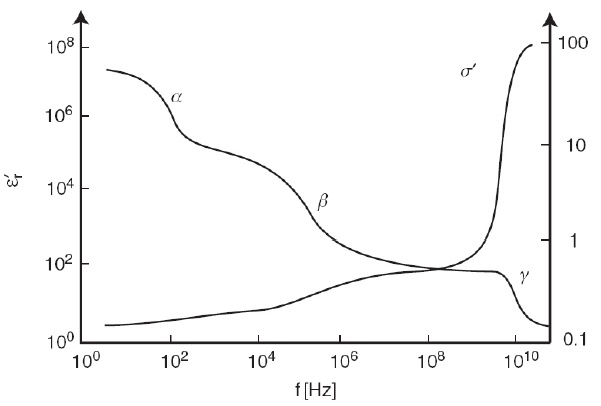
\includegraphics[width=0.8\textwidth]{./Figures/fig65}
	\caption{Variación de $\epsilon$ y $\sigma$ con la frecuencia}
	\label{fig:65}
\end{figure}

Los resultados experimentales sobre esa variación con la frecuencia se interpretan mediante estructuras y procesos pertenecientes a los tres niveles jerárquicos previos (nivel atómico-molecular, nivel de las estructuras supramoleculares y nivel celular).

Por debajo de los $100$ kHz las propiedades de conductividad de los tejidos están dominadas por la conducción de los electrolitos a través del espacio extracelular.

La conductividad promedio del tejido depende fundamentalmente de la conductividad del medio extracelular y de la fracción del volumen del medio extracelular.

Por encima de $100$ kHz la conductividad promedio depende también de la conducción de electrólitos a través del interior de las células debido a que desaparece progresivamente la barrera eléctrica establecida por las membranas celulares.

Desde el punto de vista eléctrico las membranas biológicas se comportan como una combinación en paralelo de un capacitor con un resistor.

Como la reactancia del capacitor de membrana tiende a cero a medida que aumenta la frecuencia de la corriente alterna, y el capacitor se halla en paralelo con la resistencia asociada a los canales iónicos de la membrana, la corriente alterna de alta frecuencia pasa a través del capacitor de membrana casi sin oposición, en forma de corriente de desplazamiento, eludiendo pasar a través de los canales iónicos en forma de una corriente de conducción.

Como consecuencia a altas frecuencias se produce un cortocircuito en el capacitor de membrana y se produce un aumento en la conductividad promedio.

A bajas frecuencias el tejido muestra una dispersión dieléctrica que se llama dispersión $\alpha$ y que se produce en el orden de los kHz. La dispersión $\alpha$ se debe fundamentalmente a dos procesos: 
	
	1.- La polarización de contraiones próximos a superficies cargadas eléctricamente presentes en los tejidos 
	
	2.- La polarización de grandes estructuras macromoleculares que están fijas a las membranas.

A frecuencias por debajo de las que corresponden a la dispersión $\alpha$, la permeabilidad dieléctrica relativa alcanza valores de decenas de millones. 

La conductividad por su parte varía poco en la zona de frecuencias en la que se manifiesta la dispersión

Entre $0,1$ y $10$ MHz, el tejido exhibe la dispersión $\beta$ que se debe a la variación de la carga eléctrica en las membranas celulares que se produce por un desbalance entre la corriente eléctrica en el espacio intracelular y la corriente eléctrica en el espacio extracelular.

Por encima de los $10$ MHz la impedancia de las membranas celulares se hace despreciable y las corrientes pasan tanto por el espacio intracelular como el extracelular.

Al pasar por la región correspondiente a la dispersión $\beta$ la permeabilidad dieléctrica relativa disminuye significativamente pero también es notorio el incremento de la conductividad del tejido.

A frecuencia de microondas por encima de $1$ GHz, el tejido exhibe una dispersión llamada $\gamma$ (que se centra en los $20$ GHz). Se debe a efectos de relajación de la rotación de las moléculas de agua presentes en el tejido y es el mismo fenómeno que se encuentra en el agua líquida pura. Junto con la dispersión $\gamma$ en la permeabilidad dieléctrica relativa se observa un gran incremento en la conductividad del tejido.

Tanto la conductividad como las propiedades dieléctricas de los tejidos dependen de la temperatura.

Esta descripción de las dispersiones y las variaciones en la conductividad y la permeabilidad dieléctrica en un tejido blando es una descripción basada en valores promedio, tomados sobre el volumen ocupado por la muestra de tejido estudiada. Pero en general los tejidos biológicos comprenden materiales muy heterogéneos y en un organismo inmerso en un campo externo numerosos procesos ocurren en interfaces.

Se encuentran grandes diferencias de conductividad entre, por ejemplo, los tejidos y fluidos de los vasos sanguíneos y el tejido conectivo que forma parte de los huesos.

Aunque en menor grado, pero con importantes consecuencias sobre la estimulación funcional
de fibras nerviosas, hay una diferencia de conductividad entre la sustancia gris y la sustancia
blanca en el cerebro.

Desde el punto de vista eléctrico entonces, no se puede considerar a los tejidos como un
material homogéneo.

La conductividad eléctrica y la permeabilidad dieléctrica pueden depender de la dirección en la
que se las mida, debido a la existencia de patrones morfológicos que introducen anisotropía,
tales como haces de fibras musculares, tendones, haces de fibras nerviosas y vasos sanguíneos.
Entonces, en menor o mayor grado todos los tejidos pueden presentar un comportamiento
anisótropo que se describe mediante los tensores $\bar{\bar{\epsilon}}$ y $\bar{\bar{\sigma}}$.
Para ilustrar la anisotropía en la conductividad eléctrica, se puede utilizar el esquema que
aparece en la figura \ref{fig:66}. Es un modelo eléctrico muy idealizado de un tejido, cuyas células aparecen como elipsoides alargados con sus ejes mayores paralelos entre sí. Esto define una dirección preferencial.

\begin{figure}[H]
    \centering
    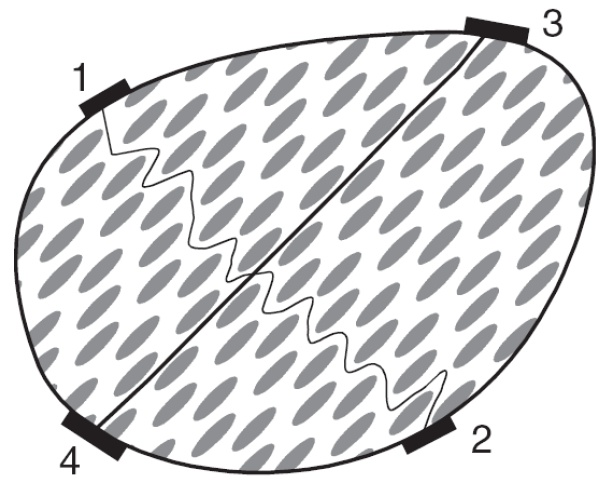
\includegraphics[width=0.5\textwidth]{./Figures/fig66}
	\caption{Modelo eléctrico de tejido}
	\label{fig:66}
\end{figure}

En la misma figura \ref{fig:66} podemos ver las dos líneas de corriente asociadas a dos pares de
electrodos en un modelo de tejido anisótropo. Se pueden ver dos pares de electrodos: el par 1-
2 que genera una corriente transversal a la dirección preferencial y el par 3-4 que genera una corriente paralela a dicha dirección.

A bajas frecuencias, las líneas que conectan los electrodos sugieren las trayectorias de la
corriente en este caso. La resistencia medida entre 1-2 es mayor que la resistencia medida entre
3-4 porque el camino que sigue la corriente transversal es más tortuoso. Este tipo de modelo
idealizado ilustra uno de los mecanismos por los cuales la conductividad eléctrica puede variar
con la frecuencia de la corriente alterna.

En la figura \ref{fig:67} vemos los Caminos de la corriente en un tejido para baja (LF) y alta (HF) frecuencia. A frecuencias lo bastante elevadas la reactancia de las membranas celulares y de las membranas de los orgánulos intracelulares prácticamente desaparece debido a que, como dijimos previamente, se cortocircuita el capacitor de membrana.

\begin{figure}[H]
    \centering
    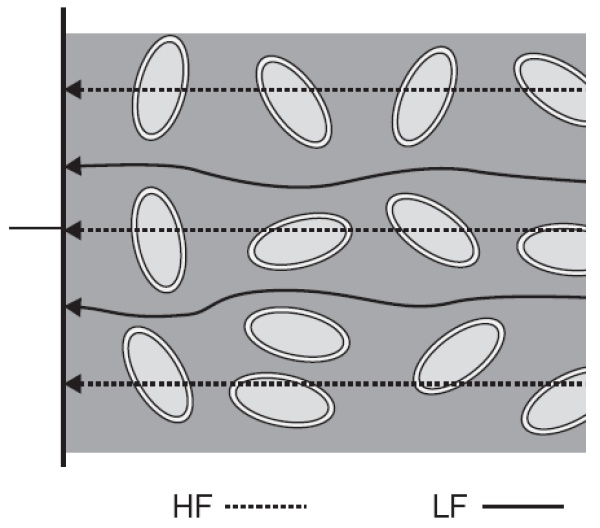
\includegraphics[width=0.5\textwidth]{./Figures/fig67}
	\caption{Caminos de corriente en alta y baja frecuencia}
	\label{fig:67}
\end{figure}

Desde el punto de vista magnético, el comportamiento de los tejidos biológicos, considerados globalmente, es por lo general mucho más simple que su comportamiento desde el punto de vista eléctrico.

Si $\ten{I}$ representa al tensor identidad y $\ten{\chi}$ representa al tensor de susceptibilidad magnética: $\ten{\mu}=\mu_{0}(\ten{I}+\ten{\chi})$
Como las componentes del tensor $\ten{\chi}$ en los tejidos biológicos en masa, diamagnéticos, son, en valor absoluto, varios órdenes de magnitud numérica inferiores a 1 (del orden de $10^{-4}$ o menor) se puede utilizar la simplificación $\ten{\mu}=\mu_{0}\ten{I}$ que implica considerar los tejidos como magnéticamente isótropos y desde el punto de vista magnético, equivalentes al medio el cual el organismo correspondiente se encuentra inmerso.

Los magnetosomas, en caso de ser necesario tenerlos en cuenta, deben tratarse por separado como estructuras mesoscópicas, es decir, a nivel dos.

En los modelos electrodinámicos a nivel de tejidos biológicos se emplean las conocidas condiciones en la frontera para los campos y las densidades superficiales de carga y de corriente de la teoría electromagnética.

En una interfaz entre dos medios o dos fases de un tejido considerado como un medio polifásico, digamos la fase 1 y la fase 2, la componente normal de la inducción magnética y la componente tangencial del campo eléctrico son continuas:

\begin{equation}
	B_{1,n}=B_{2,n} \quad \quad \quad E_{1,t}=E_{2,t}
\end{equation}


La diferencia entre las componentes normales de la inducción eléctrica a uno y otro lado de la interfaz es igual a la densidad superficial de carga eléctrica $\omega_{S}$ que pudiera hallarse en la interfaz:

\begin{equation}
	D_{1,n}-D_{2,n}=\omega_{S}
\end{equation}

Si la densidad de corriente eléctrica en la interfaz es nula, la componente tangencial del campo magnético es continua en la interfaz: 

\begin{equation}
	H_{1,t}=H_{2,t}
\end{equation}

La diferencia entre las componentes normales de la corriente eléctrica a través de la interfaz verifica una versión de superficie de la conservación de la carga:

\begin{equation}
	J_{1,n}-J_{2,n} + \dP{\omega_{S}}{t} = 0
\end{equation}

Las regiones abarcadas por las corrientes inducidas incluyen varios tipos de tejidos diferentes e interfaces entre unos y otros.

Por lo general no resulta factible tener en cuenta los detalles de la distribución espacial de las propiedades eléctricas del tejido en masa y de sus interfaces. 

Aún con el apoyo de modelos numéricos, es necesario trabajar con valores promediados.

\section{Inducción de corrientes eléctricas en el conductor de volumen de los tejidos}

Todos los sistemas de cargas aceleradas radian energía electromagnética, es decir actúan como antenas emisoras, pero no todos esos sistemas lo hacen con la misma eficiencia.

Si $\lambda$ es una longitud de onda característica emitida por un sistema de cargas aceleradas, se pueden definir dos regiones tomando como referencia la longitud $\frac{\lambda}{2\pi}$.

Cuando la distancias entre un punto de observación y el sistema emisor, es sensiblemente inferior a $\frac{\lambda}{2\pi}$, domina el patrón de campo electromagnético denominado campo cercano, mientras que si esa distancia es sensiblemente superior a $\frac{\lambda}{2\pi}$ domina el patrón denominado campo lejano o campo de radiación.

El campo cercano intercambia energía electromagnética con la fuente del campo, mientras que el campo lejano propaga como una radiación la energía electromagnética a partir de la fuente del campo, sin retornarla, a menos que sea convenientemente reflejada por algún objeto lejano.
A $50 Hz$ la longitud $\frac{\lambda}{2\pi}$ en el aire es de $960 km$. A $100$ kHz, $\frac{\lambda}{2\pi}$ es de $4800 m$. A 1 MHz, $\frac{\lambda}{2\pi}$ toma el valor $48 m$. A centenares de $GHz$, $\frac{\lambda}{2\pi}$ vale fracciones de milímetro.


\subsection{ disipación de energía y activación de tejidos excitables}

Un organismo puede interactuar y extraer energía tanto si se encuentra en el campo cercano como en el campo lejano, pero los mecanismos de interacción son diferentes en uno y otro caso.

Supongamos que un organismo se encuentra en el aire, en el campo lejano, a una distancia grande respecto de la frontera entre el campo lejano y el campo cercano de una fuente de ondas electromagnéticas. En ese caso, sobre el organismo incide una onda prácticamente plana donde el campo eléctrico y el campo magnético son ortogonales entre sí, oscilan al unísono, indisolublemente vinculados, uno con otro. Sus magnitudes se relacionan a través de la fórmula: $\dfrac{E}{H}=377\Omega$

La penetración del campo electromagnético desde la superficie hacia el interior del organismo se produce como un fenómeno de propagación de una onda que involucra a la corriente de desplazamiento $\dP{\V{D}}{t}$ y va asociada con una disipación de energía en forma térmica que puede ser muy significativa.

Como los efectos térmicos se deben a las corrientes inducidas, y no a los campos eléctricos o magnéticos interactuando directamente con las estructuras tisulares, en principio esos efectos pueden ser producidos por campos de frecuencias muy diferentes.

La densidad de energía disipada en un punto de un conductor de volumen, que se convierte localmente en energía calorífica viene, dada en función de la densidad de corriente eléctrica inducida o del campo eléctrico local, por: $\dfrac{1}{\sigma} \cdot J^{2}= \sigma\cdot E^{2}$ fácilmente reconocible como la versión diferencial de la ley de Ohm.

28
La figura \ref{fig:68} muestra los resultados de una simulación digital de la distribución de la tasa de absorción específica dentro de la cabeza de un joven irradiado por un teléfono celular a 902 MHz\footnote{Resultados numéricos debidos a Myoung Soo Kwon (Lin, 2012).}. La tasa de absorción específica aumenta a medida que ascendemos en la barra vertical pasando del azul oscuro hasta el blanco en el extremo superior (allí la tasa de absorción específica es de $1.25 W/kg$).
A la izquierda de la cabeza que aparece en la figura, a la altura del oído izquierdo, se puede apreciar la ubicación del teléfono celular y su antena.

\begin{figure}[H]
    \centering
    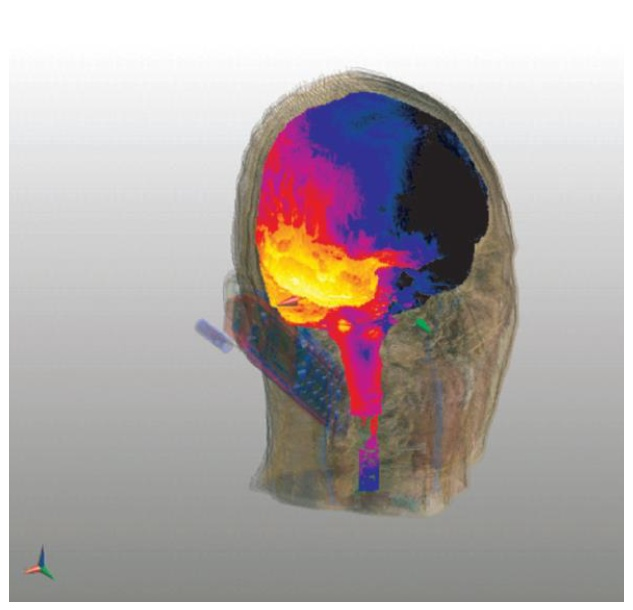
\includegraphics[width=0.7\textwidth]{./Figures/fig68}
	\caption{Perfiles de absorción de la radiación de un teléfono celular}
	\label{fig:68}
\end{figure}

Para un organismo, si la totalidad de la energía calorífica permanece en el punto en el que es entregada, la velocidad de variación de la densidad local de energía interna se relaciona con la velocidad de variación de la temperatura local $T$ , con la densidad local de corriente eléctrica $J$ y con la conductividad local $sigma$ mediante la expresión:

\begin{equation}
\rho_{m}\cdot C \cdot \dP{T}{t} =  \dfrac{1}{\sigma} \cdot J^{2} + \nabla \cdot (K_{T}\nabla T)+ F_{s} \, \rho_{s} \cdot C_{s} (T_{s}-T)+ \dot{q_{met}}
\end{equation}

Suponiendo que se conocen los valores locales de la densidad másica $\rho_{m}$, del calor específico $C$ , de la conductividad eléctrica y de la conductividad térmica $K_{T}$ local del tejido, el flujo de perfusión local de sangre $F_{S}$ , la densidad $\rho_{s}$ , el calor específico $C_{s}$ de la sangre, su temperatura $T_{s}$ y la densidad local de generación de calor por el metabolismo $\dot{q_{met}}$, esta ecuación junto con las condiciones necesarias iniciales y en la frontera, posibilita estimar el incremento de temperatura que se produce debido a la conversión en calor de la energía asociada a la corriente eléctrica.

Si los parámetros se suponen constantes y se desprecia el transporte de calor desde el lugar en el que aparece hacia las regiones vecinas y hacia la sangre, así como el aporte debido al metabolismo, se tiene para el incremento $\Delta t$ de temperatura luego de un intervalo de tiempo de breve duración $t$:

\begin{equation}
\Delta T = \left(\dfrac{1}{\rho_{m}C\sigma} J^{2} +  \dot{q_{met}} \right) t
\end{equation}

Esta expresión puede utilizarse para estimar una cota superior al incremento de la temperatura en un punto del conductor de volumen del organismo, puesto que el flujo de calor hacia otros lugares, por conducción o por convección a través de la sangre, tiene como consecuencia disminuir $\Delta T$ en igualdad de las demás condiciones.

El efecto de oír microondas, descubierto durante la segunda guerra mundial, resultó ser en última instancia de origen térmico. Consiste en sensaciones auditivas que una persona experimenta cuando su cabeza está expuesta a microondas pulsadas, como las generadas por un radar.

Un muy pequeño incremento de temperatura que se produce muy rápido en el tejido cerebral genera por expansión termo-elástica una onda acústica que viaja hacia la envoltura craneana, se refleja y transmite, y finalmente llega al oído interno siguiendo un proceso auditivo normal.
La intensidad percibida del efecto acústico, para una potencia incidente constante, depende de la duración del pulso de radar, observándose incrementos y disminuciones en la intensidad percibida asociadas a resonancias que se producen en la cavidad acústica equivalente a la cabeza humana \citep{Reilly_1998}.

Actualmente se considera que el principal mecanismo conocido por el cual las emisiones de radio y microondas producen efectos biológicos es el calentamiento de los tejidos.

En experimentos con animales se observan daños en los tejidos y otros efectos inducidos térmicamente cuando la cantidad de energía absorbida por el animal excede significativamente la cantidad de calor generada por los procesos corporales normales.

Los efectos térmicos de las radiofrecuencias o de las microondas, al mismo nivel de potencia que la generación de calor corporal en condiciones basales, parecen no representan riesgos biológicos.

Esto no descarta la posibilidad de que existan efectos no térmicos, que podría aparecer como resonancias para ciertas ventanas de frecuencia.

Para determinar en qué medida en un organismo biológico se podría producir una resonancia, el concepto de dimensión eléctrica de un sistema material resulta mucho más útil que las dimensiones geométricas tomadas por separado.

La dimensión eléctrica es un número sin dimensiones que se define en relación con una oscilación de una frecuencia dada $f$ en el material del cuerpo en el cual la velocidad de propagación de las ondas a esa frecuencia es $c$.

Se debe tener en cuenta que la frecuencia es la de la oscilación del campo externo, pero la velocidad de propagación es la del material del cuerpo.

Si $l$ es una dimensión espacial característica del cuerpo, y si $\lambda$ es la longitud de onda de la oscilación provocada por el campo externo en el material, la dimensión eléctrica se define así:

\begin{equation}
	d(f)=\dfrac{l}{\lambda}=\dfrac{l\, f}{c}
\end{equation}

Para un cuerpo con una dimensión eléctrica adecuada en presencia de un campo electromagnético externo, se puede producir una resonancia electromagnética: en un cierto lugar del conductor de volumen formado por los tejidos se puede instalar un campo eléctrico local significativamente mayor que el que aparece en ese mismo sitio para frecuencias de oscilación ubicadas fuera de la resonancia.

Como en condiciones de resonancia las estructuras biológicas que se encuentran allí localizadas interactúan con un campo oscilante de mayor amplitud, parece más verosímil esperar una transferencia de energía con consecuencias sobre los procesos metabólicos y la transferencia de señales tisulares locales y eventualmente, globales, aunque los efectos térmicos no sean significativos.

Si un organismo se encuentra dentro del campo cercano de un sistema emisor, lejos de su frontera con el campo lejano, los efectos debidos a la propagación del campo electromagnético en general pueden ser despreciados: la corriente de desplazamiento $\dPv{D}{t}$ se puede despreciar. Entonces, en el interior del organismo la ley de Ampere-Maxwell se reduce a:

\begin{equation}
\label{eq:623}
	\nabla \times \V{H} = \V{J^{i}}+\V{J_{c}}
\end{equation}

Las demás ecuaciones de la electrodinámica se mantienen incambiadas, excepto la ley volumétrica de conservación de la carga que ahora se reduce a:

\begin{equation*}
	\nabla \cdot \V{J} = 0
\end{equation*}

En este caso la disipación de energía en forma térmica no suele ser significativa y los efectos de los campos externos que se pueden observar se relacionan por lo general con la excitación de nervios, músculo esquelético y miocardio.

Teniendo en cuenta los dispositivos utilizados en el tratamiento y en el diagnóstico médico, y las características de los campos producidos por la actividad fisiológica de los organismos, consideraremos de ahora en adelante frecuencias comprendidas entre 0 y 100 kHz.

Consideremos un modelo muy simple de dos medios, aire (medio 1 de conductividad $\sigma_{1}$ y permitividad dieléctrica $\epsilon_{1}$ ) y un conductor de volumen isótropo (medio 2 de conductividad $\sigma_{2}$ y permitividad dieléctrica $\epsilon_{2}$ ).

En la interfaz $E_{1, t}=E_{2,t}$ , mientras que $D_{1,n}-D_{2,n}=\epsilon_{1}E_{1,n}-\epsilon_{2}E_{2,n}=\omega_{s}$, y $J_{1,n}-J_{2,n}=\sigma_{1}E_{1,n}-\sigma_{2}E_{2,n}=-\dT{\omega_{s}}{t}$

Suponiendo que se ha alcanzado un estado estacionario de oscilación a una frecuencia $\omega$, un factor $e^(i\omega t)$ aparece en los campos en ambos medios y en la densidad superficial de carga. Entonces $\dP{\omega_{s}}{t}=i\omega\omega_{s}$. Introduciendo esta relación en las dos ecuaciones para la componente normal del campo a uno y otro lado de la interfaz:


\begin{equation}
	i \omega \epsilon_{1} E_{1,n}-i \omega \epsilon_{2} E_{2,n}= i\omega\omega_{s}\quad \quad
	\sigma_{1}E_{1,n}-\sigma_{1}E_{1,n}=-i\omega\omega_{s}
\end{equation}


De estas ecuaciones resulta:

\begin{equation}
	(\sigma_{1} + i \omega \epsilon_{1}) E_{1,n} = (\sigma_{2}+i \omega \epsilon_{2}) E_{2,n}
\end{equation}

Si $\varphi$ es el ángulo que el campo forma con la normal a la interfaz, tenemos 

\begin{equation*}
tg(\varphi)= \dfrac{E_{t}}{E_{n}} 
\end{equation*}


Entonces, teniendo en cuenta la relación entre $E_{1,n}$ y $E_{2,n}$ obtenemos para los ángulos a uno y otro lado de la interfaz:

\begin{equation}
	tg(\varphi_{1})= \left( \dfrac{\sigma_{1} + i \omega \epsilon_{1}}{\sigma_{2}+i \omega \epsilon_{2}}\right) tg(\varphi_{2})
\end{equation}

Para frecuencias inferiores a los MHz, esto implica que el campo $\overrightarrow{E_{1}}$ en el aire tiene casi la dirección de la normal a la interfaz: el organismo distorsiona el campo eléctrico en el aire de modo que incida casi perpendicularmente a la interfaz\footnote{
Para el aire $\sigma_{1}=10^{−13}[S/m]$ y $\epsilon_{1}= 10^{-11} [F/m]$ mientras que para el conductor de volumen de los tejidos vamos a tomar $\sigma_{2}=1[S/m]$ y $\epsilon_{1}= 10^{-4} [F/m]$ para una frecuencia angular $\omega=10^{5}$ Hz. Resulta  $\left( \dfrac{\sigma_{1} + i \omega \epsilon_{1}}{\sigma_{2}+i \omega \epsilon_{2}}\right) \approx 10^{-7}$ de modo que $tg(\varphi_{1} \approx 10^{-7} tg(\varphi_{2})	$ Entonces, si $tg(\varphi_{2}) \approx 100$ (un campo $\V{E_{2}}$ en el conductor de volumen, que forma un ángulo apenas menor que $\pi/2$ con la normal a la interfaz) todavía se tiene $tg(\varphi_{1})\approx 10^{-5}$}.

La figura \ref{fig:69} esboza esta situación para un campo eléctrico oscilante que es vertical y homogéneo lejos de la interfaz con el cuerpo humano. Se advierte la distorsión, debida al cuerpo humano, en las líneas de un campo eléctrico oscilante en el aire. El sentido de las líneas se invierte cada medio ciclo de oscilación. Las líneas de campo interno y densidad de corriente eléctrica en el conductor de volumen no están a escala.

\begin{figure}[H]
    \centering
    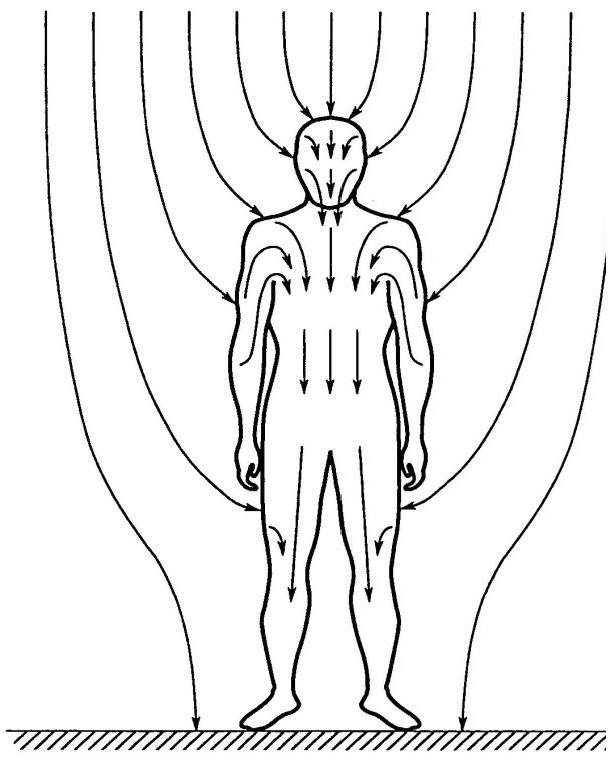
\includegraphics[width=0.6\textwidth]{./Figures/fig69}
	\caption{Campo Eléctrico en la superficie del cuerpo humano }
	\label{fig:69}
\end{figure}

Como la longitud de onda a frecuencias inferiores al MHz es muy grande respecto de la máxima distancia entre puntos del cuerpo humano, se puede suponer un campo externo variable en el tiempo, pero constante en dirección y amplitud en todas partes del espacio próximo al organismo\footnote{Los resultados de aplicar modelos más realistas \citep{Lin_2012} \citep{Polk_Postow_2006} \citep{Greenebaum_Barnes_2019} no cambian las conclusiones más importantes que se obtienen del modelo simplificado.}, siendo $\omega=2\pi\,f$ la frecuencia angular:

\begin{equation}
	E_{aire}(t)= E_{0}\,Cos(\omega\,y)
\end{equation}

Considerando para simplificar una losa transversal al campo, de conductividad $\sigma(\omega)$ y constante dieléctrica relativa $\epsilon_{r}(\omega)$, que se comportan en función de la frecuencia angular de la misma manera que se comportan esos mismos parámetros en un tejido biológico tipo.

Supondremos que la losa se puede considerar infinita en sentido perpendicular al campo oscilante.

Para los fines del presente modelo, se puede suponer que el aire que rodea la losa posee conductividad $\sigma=0$ y constante dieléctrica relativa $\epsilon \approx 1$.

La simetría de la situación física permite suponer que el campo en la losa es paralelo al campo externo, o sea es perpendicular a las caras planas de la losa. ver figura \ref{fig:610}

\begin{figure}[H]
    \centering
    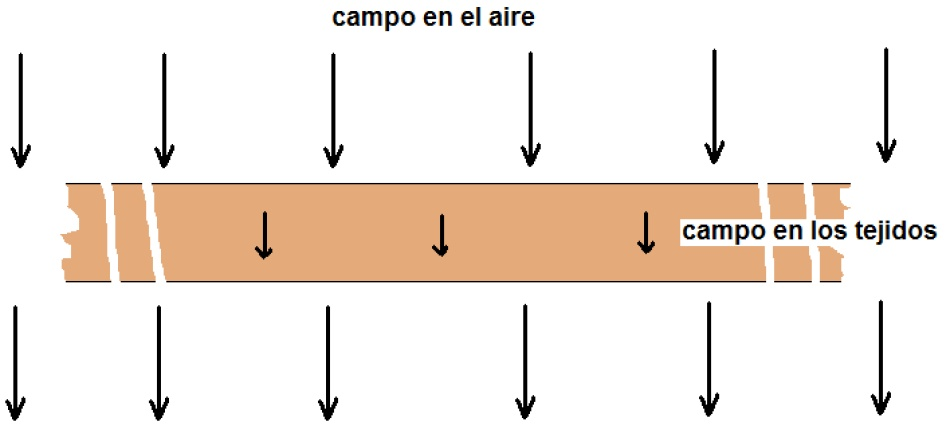
\includegraphics[width=0.8\textwidth]{./Figures/fig610}
	\caption{Modeo simplificado de campo en los tejidos}
	\label{fig:610}
\end{figure}

Si $E_{tejidos}(t)$ representa el campo en el interior de la losa que representa en este modelo a los tejidos y si $\omega_{S}(t)$ es la carga eléctrica inducida en una de las dos interfaces losa-aire (la carga inducida en la otra interfaz es $-\omega_{S}(t)$, de la condición de borde para la componente del campo eléctrico normal a la interface se obtiene:

\begin{equation}
	-\epsilon_{0}E_{aire}(t) + -\epsilon_{0}\epsilon_{r} E_{tejidos}(t) = \omega_{s}(t)
\end{equation}

La ley de conservación de la carga eléctrica suministra la relación siguiente (teniendo en cuenta que solo hay corriente de conducción en el interior de la losa, pero no en el aire):

\begin{equation}
	\sigma E_{tejidos}(t) = \dT{\omega_{s}(t)}{t}
\end{equation}

De estas dos ecuaciones se desprende: 

\begin{equation}
	\dT{E_{tejidos}}{t}+ \dfrac{\sigma}{\epsilon_{0}\epsilon_{r}}E_{tejidos}=-\dfrac{\omega}{\epsilon_{r}}E_{0}Sin(\omega\,t)
\end{equation}

\begin{sloppypar}
Luego de un transitorio cuya duración es del orden del tiempo de relajación ${\tau_{t}=\frac{\epsilon_{0}\epsilon_{r}}{\sigma}}$ se alcanza un estado estacionario de pulsación del campo eléctrico en el interior de la losa que representa a los tejidos biológicos.


Estimando el tiempo de relajación para $\sigma\approx0,5[S/m]$ y ${\epsilon_{r}\approx 50}$ resulta ${\tau\approx 10^{-9}[s]}$.
\end{sloppypar}


El campo oscilante estacionario $E_{tejidos}= ACos(\omega\,t)+BSin(\omega\,t)$ se instala entonces muy rápido.

Los coeficientes son:

\begin{equation}
	A=-(\omega\tau_{t})B \quad \quad \quad B= \dfrac{\omega\tau_{t}}{\epsilon_{R}(1+(\omega\tau_{t})^{2})} E_{0}
\end{equation}

Como para frecuencias hasta del orden de los MHz, $\omega\tau_{t}$ es mucho menor que uno, se puede despreciar $A$ frente a $B$ y se puede aproximar $B$ por $\dfrac{\omega\epsilon_{0}}{\sigma}E_{0}$ .
A partir de esta aproximación se obtiene que el campo oscilante en el interior de la losa viene dado por:



\begin{equation}
	E_{tejidos} \approx \dfrac{\omega\epsilon_{0}}{\sigma}E_{0}\, Sin(\omega\,t)
\end{equation}

De este último resultado se desprende que la densidad de corriente de conducción $J_{tejidos}=\sigma\cdot E_{tejidos}$ pulsa con frecuencia $\omega$ y posee una amplitud de oscilación $\omega\epsilon_{0}E_{0}$ \textbf{independiente de la conductividad de la losa}\footnote{Si este resultado se intentara describir desde el punto de vista de la teoría de circuitos eléctricos, habría que asumir que la fuente de fuerza electromotriz (debida al campo eléctrico externo) posee una impedancia interna tan elevada que impone una corriente independiente de la resistencia eléctrica (el conductor de volumen de los tejidos, representado por la losa) a la que alimenta.}.

Para una frecuencia de 50 Hz el campo $E_{t}$ es de un orden $10^{-8}$ veces menor que el campo $E_{0}$ en el aire.

Para una frecuencia de $1$ MHz la amplitud del campo disminuye a menos de la centésima parte.
Si el campo externo es estático, es decir si $\omega=0$, el campo eléctrico en el interior de la losa es nulo, como podía esperarse en el caso de un cuerpo conductor en equilibrio.
A frecuencias menores a $100$ kHz la membrana celular apantalla al citoplasma respecto de los campos eléctricos que puedan presentarse en el espacio extracelular.

Para una frecuencia de $50$ Hz el campo justo afuera de la célula es $10^{-5}$ veces menor que el campo en el aire, en la membrana celular es $10^{-2}$ veces menor y en el interior celular es 10-8 veces menor \citep{Lin_2012} \citep{Polk_Postow_2006} \citep{Greenebaum_Barnes_2019}.

En principio, no cabe esperar que a este nivel el campo eléctrico en el citoplasma pueda afectar los orgánulos funcionales de la célula o al ADN.

Por otra parte, se sabe ahora que tanto corrientes eléctricas débiles inducidas por un campo magnético generado por una bobina como por un campo eléctrico generado por un sistema de electrodos pueden contribuir a soldar una fractura de un hueso \citep{Polk_Postow_2006} \citep{Markov_2015}.

No obstante, este efecto de pantalla se debilita a medida que crece la frecuencia.
A frecuencias mayores a 1 MHz desaparece, porque la membrana es cortocircuitada a nivel de su capacitor.

El único efecto de pantalla remanente es el que pueda producir el conductor de volumen de los tejidos considerado en bloque.
A frecuencias inferiores a los $100$ kHz, el campo eléctrico externo no penetra casi en los tejidos biológicos, por lo cual los efectos observados se deben fundamentalmente al campo magnético externo, que penetra sin dificultad debido a que, como vimos más arriba, las permeabilidades magnéticas del aire y de los tejidos toman valores muy próximos.
El campo eléctrico inducido se conecta con el campo de inducción magnética a través de la versión integral de ley de Faraday:

\begin{equation}
	\oint \V{E}(t,\V{r}) \cdot \V{t}(\V{r})dS= -\iint \dPv{B}{t}(t,\V{r})\cdot \hat{n}(\V{t}) dS
\end{equation}

Las figuras de \ref{fig:611} sugieren lo que ocurre cuando un organismo se encuentra inmerso en un campo magnético externo oscilante y homogéneo. En ambas figuras se esbozan las líneas de campo eléctrico en el interior del cuerpo humano. A la izquierda el campo magnético es vertical y a la derecha es horizontal, como viene indicado por las flechas gruesas. En la figura a la izquierda el campo $\V{B}$se puede considerar como variable con el tiempo, vertical y homogéneo:

\begin{equation}
	\V{B}(t,\V{r}) = -B_{0}(t)\hat{e_{z}}
\end{equation}


Por el contrario, cuando el campo es horizontal y se ubica como se sugiere la figura de la derecha, el resultado de una exposición de cuerpo entero no se puede describir mediante un modelo sencillo.

\begin{figure}[H]
    \centering
    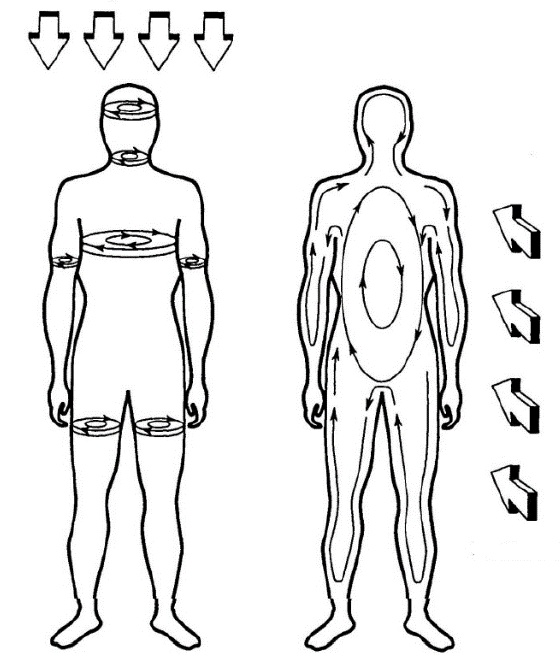
\includegraphics[width=0.7\textwidth]{./Figures/fig611}
	\caption{Corrientes inducidas en el cuerpo humano}
	\label{fig:611}
\end{figure}

Suponiendo que $\oint \V{E}(t,\V{r})\cdot\V{t}(\V{r})dS$ 

\begin{sloppypar}
se toma sobre una circunferencia horizontal de radio $r$ incluida en el conductor de volumen y que el campo eléctrico es tangencial y de igual magnitud ${E(t, r)=\V{E}(t, \V{r})\cdot \V{t}(\V{r})}$ en cada punto de la circunferencia en un mismo instante de tiempo: ${\oint \V{E}(t,\V{r})\cdot\V{t}(\V{r}) dS = 2\pi \,r \, E(t,r)}$ 

\end{sloppypar}

Por otra parte $\V{n}(\V{r})=\hat{e_{z}}$ y $\dPv{B}{t}(t, \V{r})=-\dT{B_{0}}{t}(t)\hat{e_{z}}$ 

con lo cual la integral de superficie tomada sobre el círculo de radio $r$ delimitado por la circunferencia mencionada es:

\begin{equation}
	-\iint \dP{\V{B}(t,\V{r})}{t}\cdot \V{n}(\V{r}) dS = \pi r^{2}\dT{B_{0}(t)}{t}
\end{equation}

Igualando ambas integrales se obtiene: 

\begin{equation}
	E(t, r)= \dfrac{1}{2}r\dT{B_{0}(t)}{t}
\end{equation}


Si se emplea un modelo de conductor lineal, homogéneo e isótropo de conductividad $\sigma$, la densidad de corriente inducida también es tangencial a la circunferencia y su magnitud viene dada por: 

\begin{equation}
	J(t, r)= \dfrac{1}{2}\sigma \,r \dT{B_{0}}{t}(t)
\end{equation}


Las fórmulas obtenidas para las magnitudes del campo eléctrico y de la densidad de corriente sugieren que para una misma ley de variación $\dT{B_{0}(t)}{t}$ esas magnitudes aumentan como el radio de la circunferencia.


Por ende, este modelo sencillo sugiere que, \textbf{durante una exposición de cuerpo entero a un campo externo homogéneo vertical}, los máximos de campo eléctrico y de densidad de corriente se encontrarán sobre el círculo de mayor radio que se pueda dibujar, perpendicular al vector de inducción magnética, completamente incluido en el conductor de volumen formado por el cuerpo.

En general los modelos puramente analíticos más o menos simplificados (como el que representa el cuerpo como si fuera un elipsoide prolato con eje mayor vertical) no son aplicables para estudiar los campos inducidos por exposiciones de cuerpo entero a campos magnéticos homogéneos, como las que se producen durante los estudios por resonancia magnética. Es necesario recurrir a modelos numéricos lo suficientemente detallados \citep{Lin_2012}.
La situación es muy diferente durante la estimulación funcional destinada a tratamiento médico o a diagnóstico. Ver figura \ref{fig:612}

\begin{figure}[H]
    \centering
    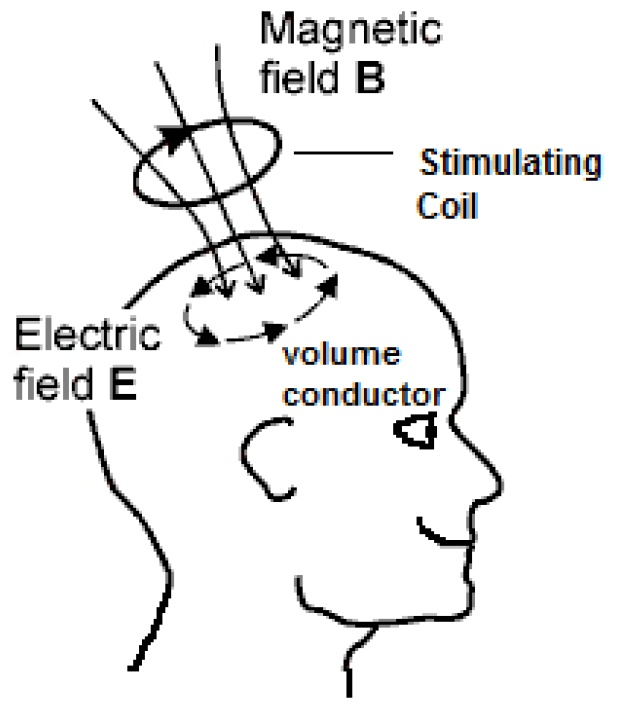
\includegraphics[width=0.5\textwidth]{./Figures/fig612}
	\caption{Corrientes inducidas en el cerebro}
	\label{fig:612}
\end{figure}

En la figura \ref{fig:612} se ilustra el método de estimulación funcional. Se advierte que el campo magnético se encuentra muy localizado. La figura fue modificada de la tesis de doctorado de Jarmo Ruohonen (1998) \citep{Jarmo_Ruohonen_1998}.

Ahora se crean campos magnéticos localizados, mediante bobinas que se sitúan próximas a la zona que se desea estimular. Ya no son campos que se puedan considerar homogéneos respecto de las dimensiones del cuerpo, pero sí son casi-estacionarios.
Se pueden expresar como el producto de un campo vectorial función de la posición $\V{F}(\V{r})$ por una función escalar $f(t)$ del tiempo:

\begin{equation}
	\V{B}(t, \V{r}) = f(t) \V{F}(\V{r})
\end{equation}

La función $f(t)$ se puede identificar con la corriente $i_{b}(t)$ que se hace circular a través de la bobina estimuladora.

El campo eléctrico local inducido viene dado por:

\begin{equation}
	\V{E}(t, \V{r}) = -\left( \dT{i_{b}(t)}{t} \right)  \V{F}(\V{r})
\end{equation}

Las corrientes inducidas generan a su vez un campo magnético propio, pero como se verá en la última parte de este capítulo, a frecuencias inferiores a $100$ kHz esos campos secundarios pueden ser despreciados.

Ahora es necesario considerar como se relaciona este campo eléctrico con la polarización de las membranas excitables de células nerviosas y musculares hasta llegar a generar la activación de la célula, manifestada por la emergencia de un potencial de acción capaz de propagarse.
Para hacer esto, partiremos de un modelo matemático simple de una fibra excitable, asimilada a un cable delgado, posiblemente curvado, cuyo interior corresponde al espacio intracelular. La membrana celular lo separa de su ambiente, formado por el resto de los tejidos.

A partir de un punto de la fibra, tomado como origen, introducimos una coordenada de posición $s$. Esta coordenada se aplica a una fibra curvada y corresponde a la longitud del arco de curva (orientado) que conecta el origen con el punto considerado.

La conexión entre el campo eléctrico inducido por el campo magnético variable y la polarización de la membrana excitable se establece a través de la \textbf{función activante}.

Esta es una función, definida para cada instante de tiempo y para cada valor de la coordenada de posición, como la derivada respecto de esa coordenada de la componente del campo eléctrico tangente a la fibra $\V{E}(t, \V{r}(s)) \cdot \V{t}(s)$


\begin{equation}
	\dP{\left\lbrace \V{E}(t, \V{r}(s)) \cdot \V{t}(s) \right\rbrace }{s} =\left( \dT{i_{b}}{t}(t) \right) \dT{(\V{F}(\V{r}(s) \cdot \V{t}(s)}{s}
\end{equation}

El vector unitario $\hat{t}(s)$ es tangente en cada punto $s$ de la fibra.

Si esta última cambia de dirección en el espacio, $\dTv{t}{s}(s)$ y aunque $\V{F}(\V{r}(s)$ sea constante a lo largo de la fibra, como podría ocurrir en ciertos casos durante una exposición de cuerpo entero, la función activante no va a ser nula y va a producir una polarización en la membrana de la fibra \citep{5627910}.

La generación de un potencial de acción en la membrana de la fibra se produce cuando en esa membrana se alcanza un patrón de polarización umbral.

Para ello una longitud mínima de membrana de una fibra, que podemos suponer se encuentra inicialmente en reposo, debe ser despolarizada por encima del denominado umbral de membrana.
Esa despolarización resulta de corrientes iónicas que cruzan la membrana desde el interior de la fibra.

Pero como no hay fuentes de corriente en el citoplasma que puedan originar este tipo de corrientes despolarizantes, la conservación de la carga eléctrica exige que las corrientes despolarizantes sean compensadas por corrientes iónicas que atraviesan la membrana, en otras partes, hacia el interior de la fibra.

El estado umbral se alcanza o no dependiendo de cómo se genere ese patrón de corrientes \citep{5627910}.

Las características del patrón generado dependen de cuánto dure y de la amplitud del estímulo, así como del estado inicial de la membrana excitable. La eficacia del estímulo depende de las características del campo inducido $\left( \dT{i_{b}}{t}(t) \right)\V{F}(\V{r})$ manifestadas a través de la función de activación $\dP{\left\lbrace \V{E}(t, \V{r}(s)) \cdot \V{t}(s) \right\rbrace }{s}$.

La figura \ref{fig:613} muestra un pulso de corriente generado en una bobina estimuladora de un equipo de estimulación magnética funcional de tercera generación junto con un patrón de magnitud de campo eléctrico inducido correspondiente a ese pulso \citep{4650502}.


\begin{figure}[H]
    \centering
    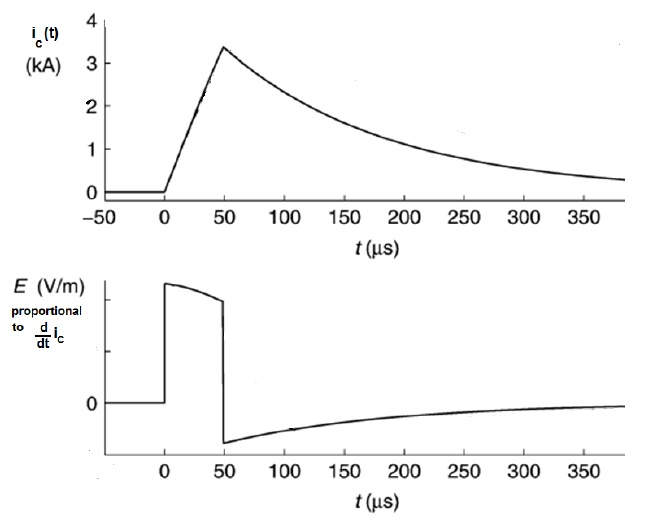
\includegraphics[width=0.8\textwidth]{./Figures/fig613}
	\caption{Pulso umbral}
	\label{fig:613}
\end{figure}

Un pulso de corriente como el que muestra la figura \ref{fig:613} es un pulso umbral cuando el campo que aparece abajo tiene una amplitud y una duración suficientes.

A menor duración, mayor tiene que ser su amplitud para alcanzar o superar el umbral.
Los resultados obtenidos se pueden graficar en un plano, ubicando la duración en las abscisas y la intensidad en las ordenadas.
Los pares duración-amplitud umbral forman una curva que se asemeja a una hipérbola con una asíntota vertical en el eje de ordenadas y una asíntota horizontal, paralela al eje de abscisas, que corresponde a una amplitud mínima, como sugiere la figura \ref{fig:614}.

Si esa amplitud mínima, conocida como reobase, no es superada, la excitación fracasa por larga que sea la duración del pulso estimulador.

La duración de un pulso cuya amplitud umbral es el doble de la reobase se denomina cronaxia.

\begin{figure}[H]
    \centering
    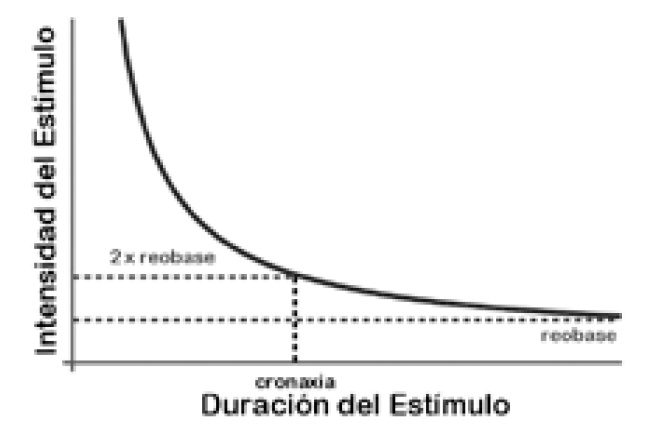
\includegraphics[width=0.7\textwidth]{./Figures/fig614}
	\caption{Relación duración vs. intensidad del estímulo}
	\label{fig:614}
\end{figure}

La curva umbral separa en primer cuadrante en dos regiones: una región de estímulos que no alcanzan el umbral, debajo de la curva, y una región de estímulos que superan el umbral, encima de la curva.

La determinación del umbral de estimulación debe hacerse en cada caso, porque la curva intensidad-duración depende de la posición y tamaño de las bobinas, de las propiedades del conductor de volumen formado por los tejidos biológicos y de la naturaleza y posición de la o las células blanco de la estimulación.

Se tienen en cuenta pequeñas variaciones aleatorias introduciendo un criterio estadístico para determinar el umbral. Por ejemplo, se considera pulso umbral cuando la excitación resulta exitosa en el 50\% de los casos para una misma amplitud y duración prefijadas en el equipo estimulador.

\section{Medición de los campos magnéticos generados por los procesos fisiológicos}

\textbf{Sus fundamentos en la teoría electromagnética de los medios continuos y  aplicación del teorema de reciprocidad.}

La actividad fisiológica del sistema nervioso (central y periférico), de los músculos esqueléticos y del corazón se acompañan de corrientes eléctricas impuestas ${J_{i}}_{T}(t, \overrightarrow{r})$ al conductor de volumen formado por los tejidos. Estas corrientes generan campos magnéticos tanto en ese conductor de volumen como en la región que rodea al cuerpo humano.

Esas corrientes y campos varían con el paso del tiempo.

Ubicando en un sitio apropiado las bobinas de un equipo receptor de señales magnéticas, las variaciones en los flujos de inducción que atraviesan las bobinas inducen en ellas fuerzas electromotrices que se pueden medir.

Como las relaciones señal-ruido son muy desfavorables, en el caso de los fenómenos magnéticos asociados a los procesos fisiológicos se emplean equipos superconductores (SQUID) y mecanismos para eliminar ruidos\footnote{Blindajes, gradiómetros o conjuntos distribuidos de bobinas conectadas a sistemas de detección multicanales.} con el fin de poder registrar magneto-cardiogramas, magneto-encefalogramas y la magneto-miografías.

\subsection{Teorema de Reciprocidad}

Veamos ahora un teorema de reciprocidad demostrado en 1895 por Hendrik Lorentz \citep{Papas_1988}, a partir del cual Robert Plonsey \citep{Plonsey_1992} pudo relacionar la fuerza electromotriz inducida en la bobina receptora con el campo de las densidades de corrientes generadas en los tejidos por la actividad fisiológica y con el denominado \textbf{campo de derivación}.

Este último campo se obtiene imponiendo una corriente eléctrica variable a los devanados de la bobina receptora, de forma tal que la variación temporal del campo magnético generado por la bobina induzca un campo eléctrico en los tejidos.

El campo de derivación se define a partir de este campo eléctrico inducido en los tejidos, como veremos a continuación.

Asumiendo las ecuaciones de Maxwell \ref{eq:ap1} y las constitutivas del medio \ref{eq:ap2} planteando como en \ref{eq:623} 

La heterogeneidad puede describirse mediante campos tensoriales dependientes del punto del espacio $\V{r}$ considerado o introduciendo un número apropiado de fases homogéneas.

Supongamos que en la región $R_{1}$ un campo de densidades de corriente impuestas $\V{J^{i}_{1}}$ genera en el espacio los campos $\V{E_{1}}$ y $\V{H_{1}}$.
En otra región $R_{2}$ un campo de densidades de corriente impuestas $\V{J_{2}^{i}}$ genera en el espacio los campos $\V{E_{2}}$ y $\V{H_{2}}$.

Supongamos, además, que ambos campos de densidades de corriente oscilan en forma monocromática a la misma frecuencia angular $\omega$ :

\begin{equation}
	\V{J_{1}^{i}}(t,\V{r}) = e^{i\,\omega\,t}\V{J_{1}^{i}}(\omega,\V{r}) \quad
	\V{J_{2}^{i}}(t,\V{r}) = e^{i\,\omega\,t}\V{J_{2}^{i}}(\omega,\V{r}) 
\end{equation}

En estado de oscilación estacionaria, los campos eléctrico y magnético oscilan a la misma frecuencia:

\begin{equation}
\begin{aligned}
	&\V{E_{1}}(t,\V{r}) = e^{i\,\omega\,t}\V{E_{1}}(\omega,\V{r}) \quad
	 \V{H_{1}}(t,\V{r}) = e^{i\,\omega\,t}\V{H_{1}}(\omega,\V{r}) \\
	&\V{E_{2}}(t,\V{r}) = e^{i\,\omega\,t}\V{E_{2}}(\omega,\V{r}) \quad
	 \V{H_{2}}(t,\V{r}) = e^{i\,\omega\,t}\V{H_{2}}(\omega,\V{r}) 
\end{aligned}
\end{equation}

Ahora todos estos campos vectoriales poseen componentes complejas: son denominados fasores vectoriales.


\subsection{Teoría electromagnética de los medios continuos}

Para un medio anisótropo (con tensores de anisotropía simétricos) y heterogéneo, el teorema de reciprocidad de Lorentz permite concluir la siguiente igualdad entre integrales de volumen:

\begin{equation}
	\int_{R}\V{E_{2}}(\omega,\V{r}) \cdot \V{J_{1}^{i}}(\omega,\V{r}) dV = 
	\int_{R}\V{E_{1}}(\omega,\V{r}) \cdot \V{J_{2}^{i}}(\omega,\V{r}) dV
\end{equation}

El producto que aparece en ambos integrandos es el producto escalar de vectores y ambas integrales se extienden a todo el espacio físico, tomando como sistema de referencia el consultorio o el laboratorio y empleando como modelo el espacio euclídeo tridimensional ${\mathbb{R}}^{3}$.

Como $\V{J_{1}^{i}}(\omega,\V{r})$ es nulo excepto en ${\mathbb{R}^{3}_{1}}$ y $\V{J_{2}^{i}}(\omega,\V{r})$ es nulo excepto en  ${\mathbb{R}^{3}_{2}}$, se obtiene la versión del teorema de reciprocidad que utilizaremos en lo que sigue:

\begin{equation}
	\int_{R^{3}_{1}}\V{E_{2}}(\omega,\V{r}) \cdot \V{J_{1}^{i}}(\omega,\V{r}) dV = 
	\int_{R^{3}_{2}}\V{E_{1}}(\omega,\V{r}) \cdot \V{J_{2}^{i}}(\omega,\V{r}) dV
\end{equation}

Esta ecuación se verifica en una situación muy general, incluso para los casos en los que se radian ondas electromagnéticas desde las regiones $\mathbb{R}^{3}_{1}$ y $\mathbb{R}^{3}_{2}$.

Se puede construir un sistema bipolar de registro y estimulación magnéticos análogo a un sistema de registro y estimulación eléctrico basado en dos electrodos.
Siguiendo una sugerencia de Baule y Mc Fee (1965) \citep{Baule_1965} en el caso magnético las superficies correspondientes a los electrodos se denominan \textbf{magnodos}.

En la figura \ref{fig:615} se muestra un conductor de volumen ocupando una región esférica.
Una bobina enrollada en un núcleo de permeabilidad elevada se conecta con el resto de un sistema que permite medir la fuerza electromotriz inducida entre las terminales \textbf{a} y \textbf{b}, e imponer corrientes eléctricas a los devanados. Las líneas que salen y entran en los extremos del núcleo y atraviesan el conductor de volumen corresponden al campo magnético que se obtiene al imponer una corriente entre las terminales \textbf{a} y \textbf{b} del devanado.
Las superficies circulares que se encuentran en uno y otro extremo del núcleo de la bobina son en este caso los magnodos.

\begin{figure}[H]
    \centering
    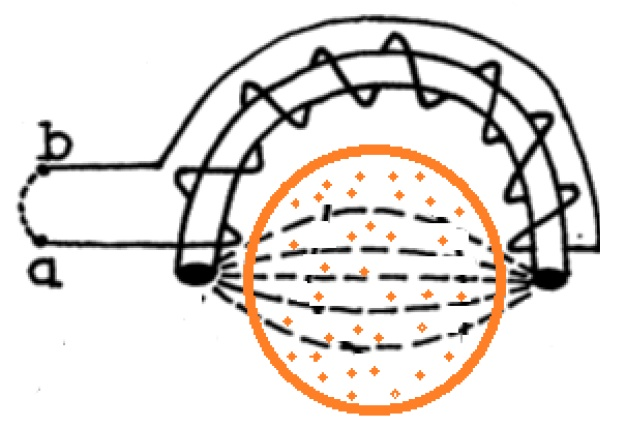
\includegraphics[width=0.5\textwidth]{./Figures/fig615}
	\caption{Conductor de volumen rodeando una esfera}
	\label{fig:615}
\end{figure}

Aplicando la fórmula de reciprocidad al caso que nos interesa, podemos tomar $\mathbb{R}^{3}_{1}=\mathbb{R}^{3}_{2}$ (siendo $\mathbb{R}^{3}_{b}$ la región ocupada por la bobina y el resto del sistema de detección) y $\mathbb{R}^{3}_{2} = \mathbb{R}^{3}_{T}$ (siendo $\mathbb{R}^{3}_{T}$ la región ocupada por el conductor de volumen de los tejidos) y obtenemos:

\begin{equation}
	\int_{R^{3}_{b}}\V{E}_{T,b}(\omega,\V{r}) \cdot \V{J_{b}^{i}}(\omega,\V{r}) dV = 
	\int_{R^{3}_{T}}\V{E}_{b,T}(\omega,\V{r}) \cdot \V{J_{T}^{i}}(\omega,\V{r}) dV
\end{equation}

La integral sobre la región $\mathbb{R}^{3}_{b}$ de la bobina involucra un producto escalar de dos campos. Uno de ellos es la amplitud vectorial de la componente armónica $\V{E}_{T,b}(\omega,\V{r})$ del campo eléctrico inducido en la bobina por el campo magnético oscilante producido, en el conductor de volumen de los tejidos, por las corrientes eléctricas asociadas a los procesos fisiológicos.

La amplitud vectorial correspondiente a estas corrientes fisiológicas es $\V{J_{T}^{i}}(\omega,\V{r})$.

El otro campo, $\V{J_{b}^{i}}(\omega,\V{r})$, es la amplitud vectorial de la componente armónica de la densidad de corriente oscilante impuesta a la bobina.

\begin{sloppypar}

A través del campo magnético que genera, la corriente impuesta a la bobina induce un campo eléctrico oscilante de amplitud vectorial ${\V{E}_{b,T}(\omega,\V{r})}$ en el conductor de volumen de los tejidos.

Dadas las frecuencias involucradas y las dimensiones geométricas de los sistemas considerados, la propagación de perturbaciones electromagnéticas se puede despreciar. Se puede trabajar con campos casi-estacionarios Plomsey y Hepner (1967) \citep{Plomsey_1967}.

Plonsey asumió una bobina filiforme. En este caso \citep{Plonsey_1972} ${\int_{R^{3}_{b}}\V{E}_{T,b}(\omega,\V{r}) \cdot \V{J_{b}^{i}}(\omega,\V{r}) dV}$ se puede aproximar por el producto ${I_{0}(\omega)V_{b}(\omega)}$.

En esta aproximación $I_{0}(\omega)$ es la amplitud de oscilación armónica de la corriente impuesta a la bobina y ${V_{b}(\omega)= \oint \V{E_{b,T}}(\omega,\V{r}(s))\cdot \V{t}(s) ds}$ es la amplitud de oscilación armónica de una fuerza electromotriz ($fem$) inducida en la bobina.
Esta $fem$ se debe al flujo magnético oscilante que atraviesa los devanados de la bobina y se origina en las corrientes eléctricas distribuidas en el conductor de volumen de los tejidos, que acompañan la actividad fisiológica del organismo.

En la integral de línea ${\oint \V{E_{b,T}}(\omega,\V{r}(s))\cdot \V{t}(s) ds}$, la función vectorial $\V{r}(s)$ representa la curva correspondiente a la bobina filiforme, mientras que $\V{t}(s)$ es el vector tangente en el punto de abscisa curvilínea $s$. Entonces: 

\begin{equation}
	V_{b}(\omega) = \dfrac{1}{I_{0}(\omega)} \int_{R^{3}_{T}}\V{E}_{b,T}(\omega,\V{r}) \cdot \V{J_{T}^{i}}(\omega,\V{r}) dV
\end{equation}

Reconstruyendo la señal de voltaje en el equipo detector:

\begin{equation}
	v_{b}(t) =  \int_{-\infty}^{+\infty} e^{i\,\omega\,t} V_{b}(\omega)\,d\omega 
\end{equation}

\end{sloppypar}

Plonsey supone:

(1) Que se puede tomar $I_{0}(\omega)=1$ para toda frecuencia angular\footnote{Lo cual equivale a que la corriente en la bobina es una delta de Dirac. En ese caso la suposición de campos casi estacionarios (o sea la posibilidad de no tener en cuenta el tiempo de propagación de las perturbaciones electromagnéticas) es difícil de justificar, aún para dimensiones de decenas de centímetros que estamos considerando.}.

(2) Que $\V{E}_{b,T}(\omega,\V{r})$ es independiente de la frecuencia en el intervalo de frecuencias donde $\V{J_{T}^{i}}(\omega,\V{r})$ no es nula\footnote{Justifica esta última hipótesis en el comportamiento del SQUID, que en el año (1971) en el que envió su trabajo para ser publicado, era un dispositivo de reciente empleo en investigaciones médicas.} y es igual a un campo denominado \textbf{campo de derivación magnética} $\V{E}_{DM}(\V{r})$.

En ese caso obtiene:

\begin{equation}
	v_{b}(t) =  \int_{R_{T}^{3}} \V{E}_{DM}(\V{r}) \cdot \V{J_{T}^{i}}(t,\V{r}) dV 
\end{equation}



Se puede observar que para un campo de densidad de corriente $\V{J_{T}^{i}}(\V{r})$ que se mantiene constante en el tiempo, en principio la integral podría no ser nula, aunque por supuesto sería constante. Pero no debería aparecer una fuerza electromotriz inducida en la bobina cuando las corrientes fisiológicas que le dan origen no varían con el curso del tiempo.

El campo de derivación, independiente siempre del tiempo, se origina en corrientes impuestas en la bobina, por lo que no tiene nada que ver con las corrientes que se observan durante la actividad fisiológica de los tejidos.

Cuando la bobina actúa como generadora de un campo magnético oscilante, induce un campo de densidades de corriente oscilante en los tejidos, que produce, a su vez, su propio campo magnético oscilante. Ese campo magnético secundario no se encuentra acotado a la región $\mathbb{R}^{3}_{T}$.

Su flujo variable puede alcanzar la bobina e inducir allí una corriente que se agregaría a la corriente impuesta e influiría a su vez sobre el campo de derivación que aparece en la fórmula para $v_{b}(t)$.

Ahora nos proponemos mostrar que:

(1)-A las frecuencias involucradas en las señales electromagnéticas asociadas a los procesos fisiológicos, el campo magnético secundario puede no ser tenido en cuenta cuando el interés se focaliza en el cálculo del campo de derivación magnética $\V{E}_{DM}(\V{r})$ producido en los tejidos por la corriente impuesta en la bobina.

(2)-Se puede deducir una fórmula para $v_{b}(t)$ análoga a la deducida por Plonsey sin necesidad de plantear las suposiciones utilizadas por este autor en su deducción.

La corriente de desplazamiento puede ser ignorada para oscilaciones cuya frecuencia angular verifica $\dfrac{\omega\epsilon}{\sigma} \ll 1$ donde $\epsilon$ y $\sigma$ son valores representativos de la permitividad dieléctrica y la conductividad del medio.

Nos proponemos mostrar que si $l$ es una longitud característica de la parte del conductor de volumen donde las corrientes inducidas por la bobina no son despreciables, entonces la condición que permite despreciar el campo magnético secundario se reduce a $l^{2}\omega\mu_{0}\sigma\ll 1$

Comencemos con el campo magnético $\V{H}_{b}(t,\V{r})$ generado cuando se impone una corriente en la bobina.
En el exterior de la región $\mathbb{R}^{3}_{b}$ y en particular en $\mathbb{R}^{3}_{T}$ , se verifica: $\Rot{H}{b}=\V{0}$

El campo magnético en los tejidos $\V{H}(t,\V{r})$ es la suma de $\V{H}_{b}(t,\V{r})$ con un campo secundario $\V{H}_{s}(t,\V{r})$ debido a las corrientes inducidas.

Si $\V{E}(t,\V{r})$ es el campo eléctrico inducido en los tejidos:

\begin{sloppypar}

\begin{equation}
	\Rot{H}{} = \sigma \V{E}(t,\V{r}) \quad \quad \Rot{E}{T} = -\mu_{0}\dPv{H}{t}(t,\V{r})
\end{equation}

Aquí consideramos un tejido homogéneo e isótropo para simplificar. Las conclusiones se aplican también al caso general.

Puesto que difieren muy poco entre sí, se tomó la permeabilidad magnética del vacío como permeabilidad de los tejidos en masa. 

Entonces:

\begin{equation}
	\nabla \times \left( \Rot{H}{}\right)  = -\mu_{0} \sigma \dPv{H}{t}(t,\V{r})
\end{equation}

Considerando un campo oscilante monocromático e introduciendo las nuevas variables de posición $\V{r}=l\V{r}_{0}$ resulta, siendo $\nabla_{0}= \dfrac{1}{l}\nabla$ y definiendo $\epsilon=l^{2}\omega\mu_{0}\sigma$:

\end{sloppypar}

\begin{equation}
	\nabla_{0} \times \left( \Roto{H}{}\right)  = - i\epsilon \dPv{H}{t}(\omega,\V{r_{0}})
\end{equation}

Introduciendo un espesor de efecto pelicular $\delta^{2}=\dfrac{1}{\omega\mu_{0}\sigma}$ se tiene: $\epsilon=\left(\dfrac{l}{\delta} \right)^{2} $

Para $l\approx 0,25 m$\footnote{$l \approx 0,25 m$ es el radio de una esfera centrada en el corazón, en cuyo interior se encuentran las densidades de corriente más intensas generadas por la actividad eléctrica del miocardio. En el caso de la estimulación magnética del cerebro, la dimensión característica es menor.}, $\omega\approx 6,28.10^{4}$ Hz, $\mu_{0}=1,257.10^{−6}\left[ \dfrac{Vs}{Am} \right]$ y $\sigma \leq 5 \left[ \dfrac{S}{m}\right]$ (una cota elevada para la conductividad de los tejidos en masa) se obtiene $\delta\geq 2,5 m$.

Entonces $\epsilon \leq 0,01$ por lo que resulta pequeño respecto de 1.

Desarrollando el campo vectorial fasor en potencias de $\epsilon$ :

\begin{equation}
	\V{H}(\omega,\V{r_{0}})=\V{H}^{(0)}(\omega,\V{r_{0}})+\epsilon \V{H}^{(1)}(\omega,\V{r_{0}})+\epsilon^{2}\V{H}^{2}(\omega,\V{r_{0}})+ \cdots
\end{equation}

\begin{sloppypar}
Sustituyendo en la ecuación ${\nabla_{0} \times \left( \Roto{H}{}\right) = - i\epsilon \dPv{H}{t}(\omega,\V{r_{0}})}$ se obtiene una secuencia de aproximaciones:
\end{sloppypar}



\begin{equation}
\begin{aligned}
	&\nabla_{0} \times \left( \nabla_{0} \times {\V{H}}^{(0)}(\omega ,\V{r_{0}})\right)  = \V{0}\\
	&\nabla_{0} \times \left( \nabla_{0} \times {\V{H}}^{(1)}(\omega ,\V{r_{0}})\right)  = {\V{H}}^{(0)}(\omega ,\V{r_{0}})\\
	&\nabla_{0} \times \left( \nabla_{0} \times {\V{H}}^{(2)}(\omega ,\V{r_{0}})\right)  = {\V{H}}^{(1)}(\omega ,\V{r_{0}})  \cdots    
\end{aligned}	
\end{equation}

De lo dicho previamente sobre el campo directamente generado por la bobina y el campo secundario generado por las corrientes inducidas, se desprende que:

\begin{equation}
	\V{H}(\omega,\V{r_{0}})=\V{H}_{b}(\omega,\V{r_{0}}) + \V{H}_{s}(\omega,\V{r_{0}})
\end{equation}

\begin{sloppypar}

La amplitud fasorial del campo secundario verifica $\Roto{H}{s}=l\sigma \V{E}(\omega ,\V{r})$ siendo en general $\Roto{E}{T} = - i \, \omega \mu_{0} l  \V{H}_{s}(\omega,\V{r}) \neq \V{0}$

Esto último junto con ${\nabla \times \V{H}_{b}(\omega,\V{r}) = \V{0}}$ nos permite inferir que ${{ \V{H}}^{(0)}(\omega,\V{r_{0}}) = \V{H}_{b}(\omega,\V{r})}$ es el campo vectorial fasor directamente generado por la bobina, mientras que el campo vectorial fasor del campo secundario viene dado por:

\end{sloppypar}

\begin{equation}
	\V{H}_{s}(\omega,\V{r_{0}})=\epsilon \V{H}^{(1)}(\omega,\V{r_{0}})+\epsilon^{2}\V{H}^{2}(\omega,\V{r_{0}})+ \cdots
\end{equation}

Como $\epsilon \ll 1$ , este desarrollo teórico sugiere que podemos despreciar el campo secundario en una primera aproximación. Desde el punto de vista práctico un campo secundario tan pequeño se confunde con el nivel de ruido magnético.

Finalmente, reconsideremos la fórmula para la señal de voltaje registrada por la bobina y debida al campo magnético generado por los tejidos.

Es conveniente comenzar con la misma fórmula utilizada por Plonsey (pero sin efectuar sus dos hipótesis):

\begin{equation}
	v_{b}(t)=\int_{-\infty}^{+\infty} e^{i\omega t}\left\lbrace  \int_{R^{3}_{T}} \dfrac{1}{I_{0}(\omega)} \V{E}_{b,T}(\omega,\V{r}) \cdot \V{J_{T}^{i}}(\omega,\V{r}) \right\rbrace d\omega
\end{equation}

Cuando a la bobina representada por la función vectorial de la longitud de arco $\V{r}(s)$ se le impone una corriente $i_{b}(t)$ ésta produce en la región $\mathbb{R}^{3}_{T}$ un potencial vector:

\begin{equation}
	{\V{A}}_{b}(t,\V{r})=\left\lbrace    \dfrac{\mu_{0}}{4\pi} \oint \dfrac{\V{t}(s)}{\vert\vert \V{r}-\V{r}(s) \vert\vert } dS       \right\rbrace  i_{b}(t)
\end{equation}

El campo eléctrico inducido en los tejidos por la corriente en la bobina viene dado por:

\begin{equation}
	\label{eq:625}
\V{E}_{b}(t,\V{r})=	-\dP{\V{A}_{b}}{y}(t,\V{r})=\left\lbrace    \dfrac{\mu_{0}}{4\pi} \oint \dfrac{\V{t}(s)}{\vert\vert \V{r}-\V{r}(s) \vert\vert } dS       \right\rbrace \dT{i_{b}}{t}(t)=\left\lbrace \dT{i_{b}}{t}(t) \right\rbrace 2\,\pi\V{\Bb{\varepsilon}}_{b}(\V{r})
\end{equation}

En esta fórmula $\V{t}(s)$ es el vector unitario tangente a la curva que representa a la bobina y la norma $\vert\vert \V{r}-\V{r}(s) \vert\vert$ expresa la distancia entre un punto $\V{r}(s)$ de la bobina y un punto $\V{r}$ perteneciente a la región ocupada por los tejidos.

Tomando la transformada de Fourier del campo eléctrico y denominando $I_{0}(\omega)$ a la transformada de Fourier de $i_{b}(t)$:

\begin{equation}
\V{E}_{b}(\omega,\V{r})= \dfrac{1}{2\pi} \int_{-\infty}^{+\infty} e^{i\,\omega\,t} \V{E}_{b}(t,\V{r})dt = i \, \omega I_{0}(\omega)\V{\Bb{\varepsilon}}_{b}(\V{r})
\end{equation}

Sustituyendo este resultado en la fórmula para $v_{b}(t)$ obtenemos:

\begin{equation}
	v_{b}(t)=\int_{-\infty}^{+\infty} e^{i\omega t}\left\lbrace  \int_{R^{3}_{T}}  \V{\Bb{\varepsilon}}_{b}(\V{r})   \, i \, \omega         \cdot \V{J_{T}^{i}}(\omega,\V{r}) \right\rbrace d\omega
\end{equation}


Como ${\int_{-\infty}^{+\infty} e^{i\omega t} \, i \, \omega \V{J_{T}^{i}}(\omega,\V{r}) d\omega = \dP{J_{T}^{i}}{t}(t, \V{r})}$ obtenemos la fórmula siguiente, análoga pero no equivalente a la obtenida por Plonsey :


\begin{equation}
	v_{b}(t)=\int_{R_{t}} \V{\Bb{\varepsilon}}_{b}(\V{r})\cdot \dP{\V{J_{T}^{i}}}{t}(t, \V{r}) dV
\end{equation}

En esta nueva expresión, el campo de derivación magnética $\V{\Bb{\varepsilon}}_{b}(\V{r})$ viene dado por:

\begin{equation}
	\V{E}_{DM}(\V{r})=\V{\Bb{\varepsilon}}_{b}(\V{r})= -\dfrac{1}{2\pi} \left\lbrace    \dfrac{\mu_{0}}{4\pi} \oint \dfrac{\V{t}(s)}{\vert\vert \V{r}-\V{r}(s) \vert\vert } dS  \right\rbrace \quad \quad (\V{r} \in R_{T}^{3})
\end{equation}


Si el campo de corrientes es estacionario, $b_{b}(t)$ se anula.

Si en un punto de los tejidos ${\dP{\V{J_{T}^{i}}}{t}(t, \V{r})}$ resulta ortogonal al campo de derivación magnética, no hay aporte a la señal captada por la bobina actuando como receptora, independientemente de la magnitud de ${\dP{\V{J_{T}^{i}}}{t}(t, \V{r})}$.

Siempre que ${\dP{\V{J_{T}^{i}}}{t}(t, \V{r})}$ no sea ortogonal al campo de derivación $\V{E}_{DM}(\V{r})$, en igualdad de las demás condiciones, donde la magnitud del campo es mayor, el aporte de las densidades de corriente a la señal captada por la bobina va a ser mayor.

Se puede introducir el campo de derivación $\V{E}_{DM}(\V{r})$ como una medida de lo que se denomina \textbf{campo de sensibilidad vectorial} del equipo de detección.


En la figura \ref{fig:616} se muestra la posición de un magnetómetro (unipolar de bobina simple) respecto de un conductor de volumen representado por una esfera. Las líneas del campo de derivación magnética aparecen esbozadas como sistemas de curvas planas concéntricas respecto de una línea que representa los puntos donde la sensibilidad es nula (donde el campo de derivación magnética se anula). Dado uno de estos planos de curvas, que son ortogonales a la línea de sensibilidad nula, cuanto más alejado del punto de corte del plano con la línea se encuentre un punto del conductor de volumen, menor es la magnitud $\vert\vert \Bb{\varepsilon}_{b}(\V{r}) \vert\vert$ de la sensibilidad.

\begin{figure}[H]
    \centering
    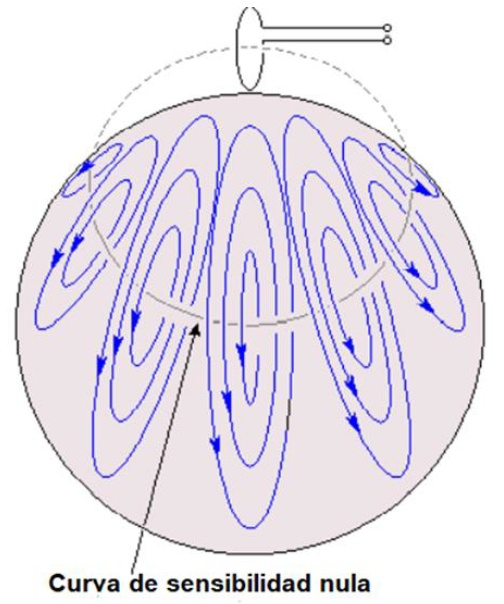
\includegraphics[width=0.5\textwidth]{./Figures/fig616}
	\caption{Magnetómetro unipolar}
	\label{fig:616}
\end{figure}


\begin{figure}[H]
  \begin{minipage}[b]{0.47\textwidth}
  En la figura \ref{fig:617} tenemos un esbozo de las líneas del campo de derivación magnética y las líneas de igual sensibilidad, también para un magnetómetro unipolar de bobina simple, pero ubicado en otra posición respecto del conductor de volumen representado ahora por un el espacio ubicado a un lado de un plano. La traza de ese plano con el plano de la figura es el eje de abscisas ($h=0$) donde se ha marcado la distancia $r$ entre el eje central de la bobina (eje de ordenadas $h$ que pasa por el centro de la bobina y es ortogonal al plano de esta última), y un punto en el conductor de volumen, cuya distancia a la superficie del conductor de volumen se representa por $h$. El eje $r=0$ (el eje $h$) es la línea de sensibilidad cero.
  
Las líneas concéntricas a este eje representan las líneas del campo de derivación magnética.
La familia de curvas que se van alejando del eje de sensibilidad cero y que en un extremo están numeradas ($100, 200, 300,\cdots, 1000,$ … hasta $10^{5}$) corresponden a líneas en cuyos puntos el campo de derivación posee la misma magnitud, es decir puntos donde el magnetómetro presenta la misma sensibilidad escalar.
  \vspace{1.5cm}
  \end{minipage}
  \hfill
  \begin{minipage}[b]{0.5\textwidth}
     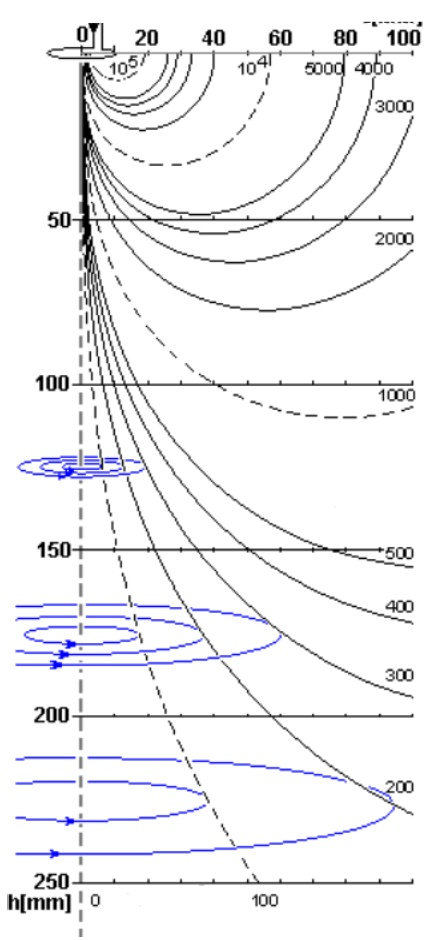
\includegraphics[width=1.10\textwidth]{./Figures/fig617}
     \caption{Derivación magnética}
	\label{fig:617}
  \end{minipage}
\end{figure}


Para la posición de la bobina que muestra la figura \ref{fig:616}, la sensibilidad escalar se puede estimar por la siguiente fórmula donde, por definición $k^{2}=\dfrac{4r_{0}r}{h^{2}+(r_{0}+r)^{2}}$, mientras $K(k)$ y $E(k)$ son, respectivamente, integrales elípticas completas de primera y segunda especie\footnote{La fórmula se obtiene a partir de la expresión para el potencial vector inducido por una corriente $i_{b}(t)$ en los devanados de una bobina circular (Nikolski, 1985; Malmivuo y Plonsey, 1995).}

\begin{equation}
	\label{eq:624}
	\vert\vert \V{\Bb{\varepsilon}_{b}}(\V{r}, h) \vert\vert = 
	\vert\vert \V{E}_{DM}(\V{r}) \vert\vert = 
	C\dfrac{1}{r}\sqrt{h^{2}+(r_{0}+r)^{2}}\left\lbrace (1-k^{2})K(k)-E(k) \right\rbrace 
\end{equation}

En la fórmula \ref{eq:624} las coordenadas del punto vienen dadas por su distancia al eje $r$ y su distancia $h$ a la superficie del conductor de volumen. El radio de la bobina es $r_{0}$ y $C$ es una constante numérica.

La fórmula \ref{eq:625}: $\V{\Bb{\varepsilon}}_{b}(\V{r})= -\dfrac{1}{2\pi} \left\lbrace \dfrac{\mu_{0}}{4\pi} \oint \dfrac{\V{t}(s)}{\vert\vert \V{r}-\V{r}(s) \vert\vert } dS  \right\rbrace$ se puede aplicar a un magnetómetro formado por un sistema de bobinas como el bipolar, esbozado en la figura \ref{fig:618}, y para magnetómetros multipolares más complejos, siempre que las conexiones entre los devanados sean las adecuadas.


\begin{figure}[H]
    \centering
    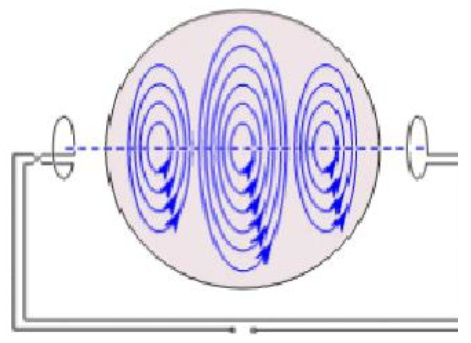
\includegraphics[width=0.6\textwidth]{./Figures/fig618}
	\caption{Esquema de un magnetómetro bipolar con bobinas ubicadas como polos opuestos.}
	\label{fig:618}
\end{figure}

En otros casos las bobinas se ubican ortogonales entre sí o del mismo lado y paralelas, compartiendo un mismo eje para formar un gradiómetro que permite atenuar gradientes espaciales no deseados en el campo magnético.

En la figura \ref{eq:619} se comparan el campo de derivación magnética de un par de bobinas opuestas (dibujo en el medio) con el campo de derivación eléctrica de un par de electrodos opuestos (dibujo de la izquierda), ubicados en un conductor de volumen esférico.


\begin{figure}[H]
    \centering
    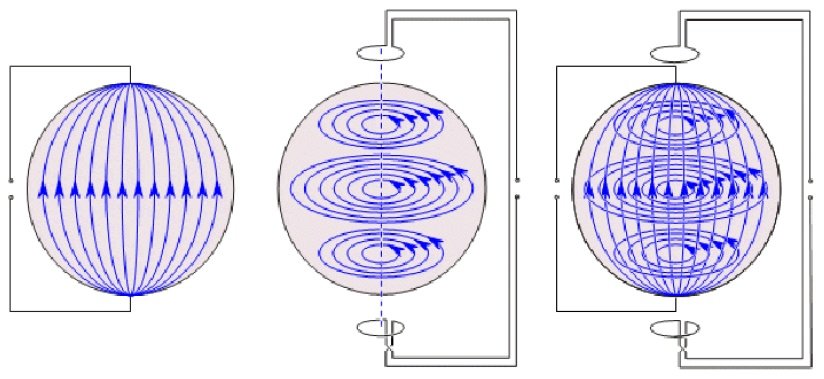
\includegraphics[width=1.0\textwidth]{./Figures/fig619}
	\caption{Distintos campos de derivación magnética}
	\label{fig:619}
\end{figure}

La tensión que aparece entre los electrodos se expresa como una integral de volumen del producto escalar de la densidad local de corriente $\V{J^{i}_{T}}(t, \V{r})$ por el vector local del campo de derivación eléctrica (Malmivuo, 2000; Suárez-Antola 2007 (a) y (b)).

La superposición de ambos campos, que se puede ver en el dibujo de la derecha, pone en evidencia la diferencia en la geometría de uno y otro campo, a lo que se añade la diferencia en sus magnitudes.

En los puntos donde el campo de derivación magnética es nulo, la magnitud del campo de derivación eléctrica suele ser máximo respecto de sus valores en los puntos próximos.

\section{Consideraciones finales}

\begin{itemize}
	\item Tanto la evidencia experimental disponible como los trabajos teóricos que plantean posibles mecanismos de interacción de los campos magnéticos con los sistemas biológicos, sugieren que los efectos no térmicos de la exposición prolongada a campos débiles pueden tener consecuencias útiles y consecuencias nocivas desde el punto biológico y médico. La posibilidad de la existencia de ventanas de baja frecuencia dentro de las cuales las interacciones se pueden amplificar por resonancias no puede ser descartada.

	\item Las normas actualmente en vigencia para limitar las exposiciones a los campos eléctricos, magnéticos y electromagnéticos se basan en la investigación de umbrales más allá de los cuales se producen efectos agudos (que aparecen a lo sumo en minutos) añadiendo luego factores de seguridad conservadores. No obstante, hay evidencia acerca de efectos de los campos magnéticos sobre el crecimiento celular, que se produce fuera de esa ventana temporal. Por otro lado, procesos más lentos dan tiempo para que los mecanismos de reparación de alteraciones estructurales, con consecuencias funcionales nocivas, puedan actuar y si lo hacen, ciertos efectos podrían no aparecer.

	\item En el caso eléctrico lo que se combina con el correspondiente campo de derivación es la densidad local de corriente, mientras que en el caso magnético lo que se combina con el campo de derivación es la derivada parcial de esa misma densidad de corriente respecto del tiempo. A partir del ejemplo de las líneas de los campos de derivación eléctrica y de los campos de derivación magnética esbozados en la figura \ref{fig:619} se comprende que, en general, la información que se obtiene midiendo fuerzas electromotrices producidas por campos magnéticos variables es complementaria respecto de la información que se obtiene midiendo el voltaje entre electrodos para una misma distribución de corriente debida a procesos fisiológicos.
\end{itemize}





